\documentclass[journal]{IEEEtran}

\usepackage{cite}
\usepackage{amsmath,amssymb,amsfonts,amsthm}
\theoremstyle{definition}
\newtheorem{criterion}{Criterion}
\usepackage{graphicx}
\graphicspath{{figures/}}
\usepackage{textcomp,xcolor,booktabs,array,url,enumitem,multirow}
\setlist{topsep=2pt,itemsep=1pt,parsep=0pt,leftmargin=*}
\usepackage{tikz}
\usetikzlibrary{positioning,arrows.meta,fit,backgrounds,automata,shapes.geometric,calc}
\usepackage{pgfplots}
\pgfplotsset{compat=1.18,table/col sep=comma}
\usepgfplotslibrary{groupplots}
\emergencystretch=1em
% float packing: many small tables, default fractions leave large gaps
\renewcommand{\topfraction}{0.92}
\renewcommand{\bottomfraction}{0.75}
\renewcommand{\textfraction}{0.07}
\renewcommand{\floatpagefraction}{0.88}
\setcounter{topnumber}{3}
\setcounter{bottomnumber}{2}
\setcounter{totalnumber}{4}
\setlength{\textfloatsep}{6pt plus 2pt minus 2pt}
\setlength{\floatsep}{4pt plus 2pt minus 2pt}
\setlength{\dblfloatsep}{6pt plus 2pt minus 2pt}
\setlength{\dbltextfloatsep}{6pt plus 2pt minus 2pt}
\setlength{\intextsep}{4pt plus 2pt minus 2pt}
\setlength{\abovecaptionskip}{3pt}
\setlength{\belowcaptionskip}{0pt}
\usepackage[normalem]{ulem}   % normalem mantiene \emph in corsivo
\usepackage{xcolor}

\newcommand{\del}[1]{{\color{blue}\sout{#1}}}  % testo rimosso: blu barrato
\newcommand{\add}[1]{{\color{red}#1}}          % testo aggiunto: rosso
\newcommand{\nongiust}[1]{{\color{red}[NON GIUSTIFICATO NEGLI ALLEGATI: #1]}}
\newcommand{\todoM}{{\color{red}[TODO: risultato M6/M7]}}

\begin{document}

\title{DIB: Managing Local MUD Policy Lifecycles with Shared IoT Traffic Evidence}
\author{Anonymous Authors}
\maketitle

%%%%%%%%%%%%%%%%%%%%%%%%%%%%%%%%%%%%%%%%%
%%%              Abstract             %%%
%%%%%%%%%%%%%%%%%%%%%%%%%%%%%%%%%%%%%%%%%
\begin{abstract}
Shared IoT traffic observations can help administrators create Manufacturer Usage Description (MUD) policies when manufacturer profiles are unavailable or outdated.
In the event of compromise, their lifecycle may require coordinated withdrawal while preserving local control over permissions.

This paper presents Device Intent Blueprint (DIB), a framework designed to facilitate the creation and sharing of MUD policies by separating shared traffic evidence from local authorization. Candidate communications enter a review queue and generate MUD rules only after local approval. \del{A shared dispute invalidates approvals, while restoration requires renewed review and preserves independent local revocations.} \add{A shared dispute triggers coordinated withdrawal while local decisions are preserved.} DIB records the approval validity and the origin of revocation, allowing disconnected sites to reconcile even after missing an entire withdrawal-and-restoration episode.

\del{To demonstrate the robustness of this framework, an exhaustive exploration of finite lifecycle models finds no property violations, and six guard-removal mutations expose distinct authorization failures. An OpenWrt/osMUD testbed demonstrates the application and withdrawal of rules. Disconnected sites reconcile through a single collapsed update; the reconciliation logic takes under 100~ms in the evaluated deployment. Experiments on three IoT traffic datasets characterize candidate selection separately from authorization. Threshold admission restricts candidates under a bounded malicious-share assumption, while score-based ordering prioritizes review. Ranking the pooled candidate set achieves a comparable review yield at matched budgets.} \add{We evaluate DIB through exhaustive lifecycle model checking, an OpenWrt/osMUD testbed, and experiments on three IoT traffic datasets. The results show that DIB works as intended: it preserves local authorization during coordinated withdrawal and recovery, reconciles disconnected sites in about 70~ms on average in the evaluated deployment, and supports flexible candidate selection.} \del{These results support configurable candidate selection within a lifecycle that preserves local decisions during coordinated recovery.}\add{Overall, the tests confirm that DIB works as intended, with reconciliation taking about 70~ms on average in the evaluated deployment.}
\end{abstract}

\begin{IEEEkeywords}
IoT security, Manufacturer Usage Description, distributed network management, access policy management, policy lifecycle.
\end{IEEEkeywords}

%controllare introduzione concetti
%testebed reale migliora articolo (?)

%active ricorsivo

%check lifecycle and reconciliation stato dell'arte

%%%%%%%%%%%%%%%%%%%%%%%%%%%%%%%%%%%%%%%%%
%%%      Section I: Introduction      %%%
%%%%%%%%%%%%%%%%%%%%%%%%%%%%%%%%%%%%%%%%%
\section{Introduction}
\label{sec:introduction}
Internet of Things (IoT) devices rely on network services for updates, remote control, and data exchange. Restricting their communications to the services they need can limit their exposure and the network activity of compromised devices~\cite{mirai,hernandezramos2021mudreview}. To support this approach, the Internet Engineering Task Force (IETF) standardized Manufacturer Usage Description (MUD) in RFC~8520~\cite{rfc8520}. This standard involves MUD files, describing a device's intended communications, and MUD managers, which translate this description into access-control rules for the local networks.

Since manufacturer profiles may be unavailable or become outdated as firmware and cloud services change~\cite{hernandezramos2021mudreview,allowlistvariability}, traffic observations can help administrators draft or update these profiles, and reports from other networks provide additional evidence when local observations remain limited. However, a service used in one network may be unnecessary in another, and observed traffic may include communications generated by compromised devices~\cite{allowlistvariability,mirai}. Therefore, administrators must decide which proposed rules to apply in their own networks.

These decisions are part of a policy lifecycle. For instance, considering a camera without a manufacturer profile: two networks observe the same cloud service, and an administrator uses their reports to approve a local rule. If a contributor later disputes that service, the participating networks must withdraw the associated permissions. Once the dispute is resolved, the system must distinguish dispute-induced withdrawal from independent local revocation. It must preserve this distinction when reconciling a network that was disconnected throughout the episode.

To overcome this limitation, this paper proposes \emph{Device Intent Blueprint (DIB)}, a framework for managing locally authorized MUD policies based on shared IoT traffic observations. We call each independently administered network a \emph{site}. DIB groups observations into \emph{endpoint facts}, each of which identifies a (i) device type, (ii) communication direction, (iii) protocol, (iv) peer, and (v) port. The observations and contributor reports supporting a fact form its \emph{evidence}, and a \emph{registry} stores that evidence alongside separate records of each site's policy decisions.
% Non ho capito molto bene cosa voglia dire la frase sopra.

DIB separates candidate selection from authorization. Selected facts enter the MonitorOnly state, where administrators can review them without creating MUD rules.
Once an administrator approves locally, a fact is moved to the active state, and it can be exported to other sites. A shared dispute invalidates approvals; restoration requires renewed review and preserves local revocations. Ordered updates reconcile sites that missed intermediate changes.


Existing approaches cover profile extraction, evidence sharing, and coordinated authorization (see Table~\ref{tab:positioning}). DIB addresses recovery across independent authorities by combining deny-overrides and a last-writer-wins pending register with explicit approval validity and revocation origin. Together, these records determine whether a recovering site must return a fact to review or retain an independent local veto.

To conclude, the main contributions of this paper are:
(1)~a policy lifecycle and reconciliation mechanism that preserves local authorization during shared withdrawal and recovery, including after missed episodes;
(2)~a registry and distributed prototype, evaluated through finite-state verification, controlled ablations, recovery experiments, and OpenWrt/osMUD enforcement;
(3)~a matched evaluation on three IoT traffic datasets that distinguishes the effects of candidate admission and review ordering.

%the goal is
% to validate this contribution we did

The remainder of this paper is organized as follows. Section~\ref{sec:related-work} reviews related work. Section~\ref{sec:threat} defines the system model, design goals, and threat model. Section~\ref{sec:design} presents DIB. Sections~\ref{sec:impl} and~\ref{sec:eval} describe the proposed implementation and its evaluation. Finally, Section~\ref{sec:discussion} discusses implications and limitations.



%%%%%%%%%%%%%%%%%%%%%%%%%%%%%%%%%%%%%%%%%
%%%     Section II: Related Work      %%%
%%%%%%%%%%%%%%%%%%%%%%%%%%%%%%%%%%%%%%%%%
\section{Related Work}
\label{sec:related-work}

RFC~8520 leaves the local application of MUD recommendations to the network administrator and calls for policy updates to respect deployment-specific approval flows~\cite[Secs.~1.1 and~1.8]{rfc8520}. A parallel IETF effort standardizes MUD URL reissuance~\cite{mudacceptableurls}, which addresses authority over manufacturer URL updates. DIB governs operator-approved facts derived from traffic observations. Prior work extracts or enforces profiles from local traffic within one administrative domain~\cite{clearasmud, hamzatdsc, mudflow, CornoMannella2023GatewayMUD, osmud, mudscope} rather than governing observations shared across domains.

Threat-intelligence sharing platforms (MISP, STIX), contributor reputation systems~\cite{wagner2016misp, stix21, eigentrust, trustsurvey}, and collaborative IoT learning (CoLearn, D\"IoT, IoT Inspector)~\cite{colearn,ndiot2019, iotinspector, vasilomanolakis2015collaborative} aggregate evidence, traffic models, or anomaly reports. These approaches share information rather than grant network access, and therefore specify no withdrawal semantics for permissions already installed at a recipient.

Policy-based management and intent frameworks address policy specification, conflicts, and configuration~\cite{pbnm,rfc9315,alshaer2004firewall,chowdhary2022intent,pipeconf2022,vergutz2023data}. POLARIS~\cite{polaris} lets resource owners decide access from verifiable attributes and binds access to sessions. FIDEM~\cite{fidem} verifies device--MUD-class binding and propagates profile updates through URL reissuance or signature-change checks. Their workflows address identity-based access and profile authenticity, respectively. DIB assumes established identities and specifies how shared withdrawal invalidates per-site approvals, how restoration preserves local vetoes, and how sites reconcile after missed episodes. Dynamic and security-tested MUD profiles~\cite{blockchainmud,matheu2019mudtesting} also motivate profile evolution.

The deny-overrides combining rule in XACML and policy frameworks~\cite{xacml3, ponder} resolves conflicting decisions during policy evaluation. DIB retains the origin of a revocation across updates so that a shared restore preserves a local denial. Zanzibar~\cite{zanzibar} addresses stale authorization through consistency tokens in a globally coordinated service, where one authority both grants and revokes. DIB propagates withdrawal to sites that grant permissions independently and reconciles unreachable sites after reconnection. Its pending target follows a last-writer-wins register~\cite{crdt}, with local guards preserving revocation origin.

\textcolor{red}{Paragrafo qui in cui enfatizzi in cosa DIB è diverso/migliore e cosa pensi possa portare alla community scientifica.} Table~\ref{tab:positioning} compares the closest related systems. 

\begin{table}[ht]
\centering
\caption{Positioning against the closest related systems.
``Disconnected'': What happens to a participant who misses a withdrawal?
``Origin'': whether shared restoration distinguishes dispute-induced revocation from independent local revocation.}
\label{tab:positioning}
\scriptsize
\setlength{\tabcolsep}{3pt}
\renewcommand{\arraystretch}{1.05}
\begin{tabular}{@{}>{\raggedright\arraybackslash}p{1.52cm}>{\raggedright\arraybackslash}p{1.32cm}>{\raggedright\arraybackslash}p{1.84cm}>{\raggedright\arraybackslash}p{1.56cm}>{\raggedright\arraybackslash}p{1.26cm}@{}}
\toprule
Approach & Authority & Propagated & Disconnected & Origin \\
\midrule
MUD extraction~\cite{clearasmud, hamzatdsc, mudscope} & single domain & none (no sharing) & n/a & n/a \\
Evidence sharing~\cite{wagner2016misp, stix21, colearn} & recipient & reports, models & unspecified & not modeled \\
FIDEM~\cite{fidem} & manufacturer & profile, URL updates & re-check on reconnect & n/a \\
POLARIS~\cite{polaris} & resource owner & bound sessions & session expiry & n/a \\
Zanzibar~\cite{zanzibar} & one global service & consistency tokens & blocks on staleness & single origin \\
\textbf{DIB} & \textbf{each site} & \textbf{ordered lifecycle targets} & \textbf{stale grant voided} & \textbf{preserved} \\
\bottomrule
\end{tabular}
\end{table}



\section{System Model, Design Goals, and Threat Model}
\label{sec:threat}

We consider a closed consortium of independently administered sites. Each site has a local operator, a MUD manager, and a gateway. Sites send traffic observations to a shared \emph{evidence service}, which holds the shared part of the registry, selects candidate endpoint facts, and distributes lifecycle updates such as disputes and restorations; each site keeps its own decisions (Fig.~\ref{fig:architecture}).
% SRC: "registry" introdotto a tex:78; evidence service vs registry tex:190, :231. Recap riunione: "iniziare con gli obiettivi di design prima di costruire il modello".

\subsection{Design Goals}
\label{subsec:goals}
Each goal is stated with the observation that would refute it.

\begin{itemize}
\item \textbf{G1: Evidence-based proposals.} For a device type whose manufacturer profile is unavailable or outdated, a site receives candidate endpoint facts derived from other sites' observations, and fewer candidates reach review than the facts reported in total. \emph{Refuted if} shared proposals match the receiver's traffic no better than its own observations at cold start, or if candidate selection does not reduce the review volume.
% SRC: G1 attuale tex:153 (frase rotta: audit/19:98,136; piano:55); "unavailable or outdated" tex:48, :74; G3 commentato "Review workload" tex:158.

\item \textbf{G2: Conditional admission protection.} A fact enters a site's review queue only if its shared evidence passes an admission rule. If malicious contributors make up at most a bounded fraction of the sites that observe a device type (assumption AS2 below), no fact reported only by them passes the rule. Passing does not establish that a communication is benign or necessary. \emph{Refuted if} a fact reported only by malicious contributors within that bound is admitted.
% SRC: G2 attuale tex:156; versione commentata tex:163; Recap: "specificare che i fatti devono superare una certa soglia per essere importati"; "protezione condizionale per l'ammissione".

\item \textbf{G3: Local authorization with conservative withdrawal.} In every reachable state, a fact produces a MUD rule at a site only if that site's operator approved it and no later dispute or restoration has voided the approval; nothing shared creates an approval, and local actions never change another site's records. A dispute removes the rule at every site, upon reconciliation if the site is unreachable; a restoration returns the fact to review and preserves local revocations, also at sites that missed the episode. \emph{Refuted by} a rule without a valid approval, a peer record changed by a local action, a disputed fact exported after reconciliation, or a local revocation erased by a restoration.
% SRC: G3 attuale tex:157 ("tautologico", commento tex:168); G4 attuale tex:160-161 e G4 commentato tex:160 fusi qui;
% SRC: Recap: "il revoking e' automatico quando ci sono dispute in rete". Intro: tex:76, :82.
\end{itemize}

G3 is a lifecycle invariant, formalized as I1--I3 in Sec.~\ref{subsec:lifecycle}; it imposes no deadline on withdrawal, and Sec.~\ref{sec:netem-results} measures how long withdrawal takes at reachable sites under emulated delay and loss. G1 and G2 concern candidate selection, which affects what operators review but never what a gateway enforces. Sections~\ref{sec:lifecycle-results}, \ref{sec:scalability-results}, and~\ref{sec:netem-results} test G3, Sec.~\ref{sec:utility-results} G1, and Sec.~\ref{sec:security-results} G2.
% SRC: "due rischi" tex:166 riformulati; nessun limite di tempo tex:332.

\subsection{Roles, Trust Boundary, and Assumptions}
\label{subsec:trust}
Members submit observations, read their own candidates, and send \emph{dispute notices}, i.e., requests to withdraw a fact. Each site's operator alone approves, revokes, and restores facts at that site. A consortium administrator alone performs global restoration after a dispute. The evidence service aggregates evidence, selects candidates, and orders and distributes lifecycle updates; it is trusted for this, not to authorize. Each site's MUD manager and gateway apply only that site's policy.
% SRC: tex:174, :184; "report message" -> "dispute notice" (piano:59,78; Recap: rivedere "report message").

The boundary of each site's administrative domain (dashed boxes in Fig.~\ref{fig:architecture}) is the only place where authorization is created. Inputs that cross it from outside, such as observations, candidates, disputes, and restorations, can at most place a fact in review or withdraw its rule; they cannot install a rule. The goals rely on six assumptions:
\begin{itemize}
\item \textbf{AS1 (Authenticated identities and roles).} Every request is bound to an identity and the role rules above are enforced, e.g., through mutual Transport Layer Security (TLS) with X.509 certificates bound to site identifiers. The finite models and lifecycle experiments use trusted caller identities, so G3 holds conditionally on AS1.
\item \textbf{AS2 (Bounded per-type malicious share).} For every device type $d$, the sites whose reports for $d$ are malicious---colluding members and honest sites that report the traffic of compromised devices---make up at most a fraction $f_s$ of the sites contributing evidence for $d$ (formalized in Sec.~\ref{sec:scoring}). Because that population is derived from submitted evidence, membership governance must verify which device types each member operates; the prototype does not perform this check. Only G2 depends on AS2.
\item \textbf{AS3 (Aligned labels).} Sites map device labels to common device types before submitting evidence.
\item \textbf{AS4 (Trusted local domain).} A site's operator, MUD manager, and gateway act on behalf of that site; misuse of a local approval or revocation is an insider action.
\item \textbf{AS5 (Policy authority).} A gateway applies only policies signed by its own site's authority, whose key neither peers nor the evidence service hold; the testbed uses unsigned policies (Sec.~\ref{sec:impl}).
\item \textbf{AS6 (Eventual delivery).} Every site eventually reconnects and retrieves the updates it missed, after an unbounded time; network faults lose messages but do not forge them.
\end{itemize}
% SRC: AS1 tex:172, :184; audit/13:9-17. AS2 tex:172; ES_d autodichiarato audit/08:94 (H2), :237; A1 nella quota audit/09:43;
% SRC: lista tipi solo su /attest e /dispute audit/13:190,202. AS3 tex:172. AS4 tex:179. AS5 tex:174, :427; audit/01 D14.
% SRC: AS6 tex:332, :530; audit/07:84.

\subsection{Adversary Model}
\label{subsec:adversary}
The adversary may control colluding members, which submit arbitrary observations and dispute notices; compromise devices inside honest sites; obtain extra identities when membership control fails; and disconnect sites for finite periods. It cannot impersonate a member (AS1), act as an operator (AS4), or sign a site's policy (AS5). We consider four threats:
(i)~\textbf{A1 (Poisoned observations)}: an honest site reports real flows of a compromised device; (ii)~\textbf{A2 (Fabricated evidence)}: members report traffic that did not occur, within the share of AS2 or, in stress tests, with fabricated identities beyond it; (iii)~\textbf{A3 (Low-and-slow drift)}: device behavior changes gradually across sites, so legitimate and malicious change produce the same observations; and (iv)~\textbf{A4 (Dispute abuse)}: members send unfounded dispute notices to withdraw legitimate rules. A1 and A2 target G2, A3 targets G1 and G2, and A4 targets availability. Disconnections are faults covered by AS6. Section~\ref{subsec:security-analysis} relates each threat to the mechanisms that address it.
% SRC: A1-A3 tex:177 (refuso "A1 tests -----." eliminato; audit/19:137); A3 tex:179; A4 tex:179 ("raise baseless disputes"), :539-541, :675.
% SRC: Recap: "possibilita' di compromettere il sistema attaccando due siti simultaneamente" = A4 con conferma a due siti.

\textbf{Out of scope.} We do not address misuse by a site's own administrator (AS4); compromise of a certificate authority or of a signing key; the quality of operator decisions; confidentiality of shared evidence; binding of a physical device to its device type; denial of service against the evidence service; a time bound for withdrawal; or traffic whose peer names are hidden by encrypted DNS or Encrypted Client Hello (Sec.~\ref{sec:discussion}).
% SRC: tex:179; piano:153; audit/13:29-33; tex:465, :671; tex:109; tex:677; tex:332, :675; tex:679.


\section{Proposed Approach}
\label{sec:design}
DIB comprises a shared evidence service and independently administered site services (Fig.~\ref{fig:architecture}). The evidence service receives observations and distributes candidates and ordered lifecycle updates. Each site retains its decisions, operator interface, and MUD exporter. Its service applies shared updates, preserves local revocations, and exports approved endpoint facts to the MUD manager.

\begin{figure*}[ht]
\centering
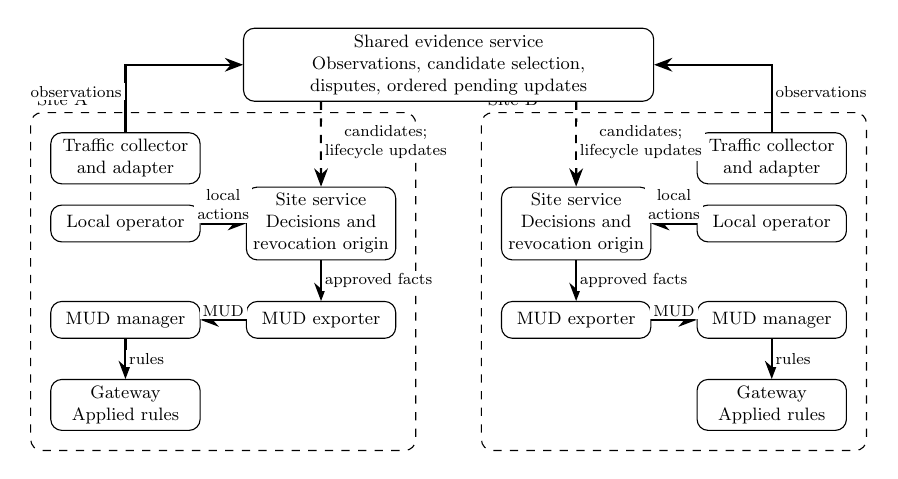
\begin{tikzpicture}[scale=0.72,transform shape,>=Stealth,
 component/.style={draw,rounded corners,align=center,font=\small,minimum height=0.65cm,text width=2.4cm,fill=white},
 flow/.style={->,thick},
 event/.style={->,thick,dashed},
 labeltext/.style={font=\footnotesize,align=center,fill=white,inner sep=1.5pt}]
\node[component,text width=7cm,minimum height=0.95cm] (evidence) at (0,0)
 {Shared evidence service\\Observations, candidate selection, disputes, ordered pending updates};
\foreach \side/\inner/\outer/\name in {a/-2.25/-5.7/A,b/2.25/5.7/B}{
 \node[component] (collector-\side) at (\outer,-1.65) {Traffic collector\\and adapter};
 \node[component] (operator-\side) at (\outer,-2.80) {Local operator};
 \node[component,minimum height=0.95cm] (site-\side) at (\inner,-2.80) {Site service\\Decisions and\\revocation origin};
 \node[component] (export-\side) at (\inner,-4.50) {MUD exporter};
 \node[component] (manager-\side) at (\outer,-4.50) {MUD manager};
 \node[component] (gateway-\side) at (\outer,-6.00) {Gateway\\Applied rules};
 \draw[flow] (operator-\side) -- node[labeltext,above]{local\\actions} (site-\side);
 \draw[flow] (site-\side) -- node[labeltext,right]{approved facts} (export-\side);
 \draw[flow] (export-\side) -- node[labeltext,above]{MUD} (manager-\side);
 \draw[flow] (manager-\side) -- node[labeltext,right]{rules} (gateway-\side);
 \begin{scope}[on background layer]
  \node[draw,dashed,rounded corners,fit=(collector-\side)(site-\side)(operator-\side)(gateway-\side)(export-\side),inner sep=0.25cm,
  label={[font=\small,anchor=south west]north west:Site \name}] {};
 \end{scope}
}
\draw[flow] (collector-a.north) |- node[labeltext,pos=0.30,left]{observations} (evidence.west);
\draw[flow] (collector-b.north) |- node[labeltext,pos=0.30,right]{observations} (evidence.east);
\draw[event] ([xshift=-2.25cm]evidence.south) -- node[labeltext,right,pos=0.47]{candidates;\\lifecycle updates} (site-a.north);
\draw[event] ([xshift=2.25cm]evidence.south) -- node[labeltext,right,pos=0.47]{candidates;\\lifecycle updates} (site-b.north);
\end{tikzpicture}
\caption{DIB's distributed architecture. Dashed boxes delimit local administrative authority. Solid arrows carry observations, local decisions, and policy output; dashed arrows carry shared candidates and lifecycle updates, which disconnected sites retrieve on reconnection. The MUD manager and gateway may be co-located, as in the OpenWrt testbed.}
\label{fig:architecture}
\end{figure*}


\subsection{Records and Operational Flow}
\label{subsec:endpoint-facts}
For device type $d$, an endpoint fact is $f=(d,e)$, where $e=(\text{direction},\text{protocol},\text{peer},\text{port})$. The peer is a Fully Qualified Domain Name (FQDN) or remote IP address. Before scoring, adapters associate observed names with addresses and normalize protocol labels. Names come from DNS records or HTTP/TLS metadata, depending on the dataset; the remaining fields come from the flow's direction, protocol, and port. Scoring uses outbound communications because the evaluated captures predominantly contain device-initiated traffic. The exporter can also generate return-flow entries.

The \emph{DIB registry} is the logical record model for shared evidence and per-site decisions. The single-registry implementation stores both in one service. In the distributed prototype, the shared evidence service holds only shared records; each site stores its own decisions (Sec.~\ref{sec:scalability-results}). Shared records contain observations, reporting sites, timestamps, and attestations. The contribute operation deduplicates submissions; attest records a positive site assessment. \emph{Local} evidence fails admission; \emph{Corroborated} evidence meets the endpoint, reporting-site, score, and dispute checks for review (Sec.~\ref{sec:scoring}). Three distinct positive attestations promote an undisputed Corroborated record to \emph{Consortium-attested}. These labels establish neither benignity nor permission to communicate.

Site-local records hold decisions and their revision history. A \textsc{query} stages an admissible fact as MonitorOnly if the site has no record, or returns its existing decision; it is therefore not a read-only operation. MonitorOnly places a proposal in the operator's review queue without generating a network rule. Local approval is recorded through \textsc{operator-commit} (a local commit), the only operation that authorizes export. Decision history records lifecycle events and the resulting state, actor, time, and reason where supplied, allowing restoration to distinguish a local veto from shared withdrawal.

\textbf{From observations to a MUD rule.} To provide an example of an observation that could become an endpoint fact, we can assume having two different sites (A and B), both having inside their network an IP Camera. In this example, the two sites report TCP traffic to \texttt{api.vendor.example} on port 443. Once admitted, the fact enters site A's review queue as MonitorOnly. An \textsc{operator-commit} moves it to Active, and the exporter emits an access-control entry (ACE) matching the destination DNS name and TCP port in the from-device access-control list (ACL), which the MUD manager resolves and installs. Site B requires its own approval. Table~\ref{tab:record-example} summarizes the outcomes of this example.
On the other side, withdrawal regenerates the site's policy, which the gateway must apply to remove installed permissions. Table~\ref{tab:transitions} specifies the recovery transitions.

\begin{table}[ht]
\centering
\caption{Illustrative records and export for the camera example. Field groups summarize stored information, not an API serialization.}
\label{tab:record-example}
\scriptsize
\begin{tabular}{@{}p{1.5cm}p{5.6cm}@{}}
\toprule
Record & Example contents \\
\midrule
Endpoint fact & (camera, out, TCP, \texttt{api.vendor.example}, 443) \\
Evidence & Reporters: sites A and B; observation timestamps and counts; computed admission score \\
Site A decision & Active after A's commit; valid approval; commit event in decision history \\
Site B decision & MonitorOnly; no approval; no exported rule \\
Site A MUD ACE & Destination DNS name \texttt{api.vendor.example}; IP protocol 6; TCP destination port 443; forwarding accept \\
\bottomrule
\end{tabular}
\end{table}

\subsection{Site-Local Authority Lifecycle}
\label{subsec:lifecycle}
\begin{figure}[t]
\centering
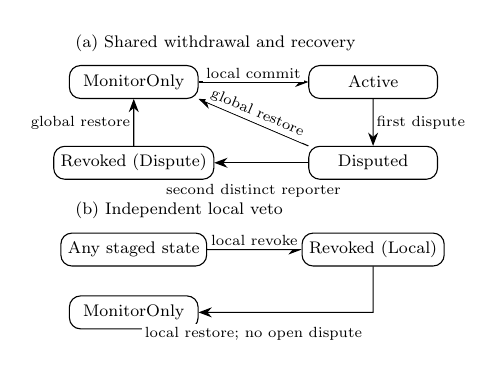
\begin{tikzpicture}[scale=0.76,transform shape,>=Stealth,
box/.style={draw,rounded corners,align=center,minimum width=2.15cm,
minimum height=0.55cm,font=\footnotesize},
lab/.style={font=\scriptsize,fill=white,inner sep=1.5pt}]
\node[font=\footnotesize,anchor=west] at (-1.1,0.65) {(a) Shared withdrawal and recovery};
\node[box] (review) at (0,0) {MonitorOnly};
\node[box] (active) at (4.0,0) {Active};
\node[box] (revoked) at (0,-1.35) {Revoked (Dispute)};
\node[box] (disputed) at (4.0,-1.35) {Disputed};
\draw[->] (review)--node[lab,above]{local commit}(active);
\draw[->] (active)--node[lab,right]{first dispute}(disputed);
\draw[->] (disputed)--(revoked);
\node[lab] at (2,-1.82) {second distinct reporter};
\draw[->] (revoked)--node[lab,left]{global restore}(review);
\draw[->] (disputed.north west)--node[lab,sloped,above]{global restore}(review.south east);
\node[font=\footnotesize,anchor=west] at (-1.1,-2.15) {(b) Independent local veto};
\node[box] (source) at (0,-2.8) {Any staged state};
\node[box] (local) at (4.0,-2.8) {Revoked (Local)};
\draw[->] (source)--node[lab,above]{local revoke}(local);
\node[box] (reviewb) at (0,-3.85) {MonitorOnly};
\draw[->] (local.south)--(4,-3.85)--(reviewb.east);
\node[lab] at (2,-4.2) {local restore; no open dispute};
\end{tikzpicture}
\caption{Recovery paths for an admitted fact. A local veto can be recorded from MonitorOnly, Active, Disputed, or Revoked (Dispute), and survives global restore. Panel (a) shows withdrawal from Active; all guards are in Table~\ref{tab:transitions}.}
\label{fig:lifecycle}
\end{figure}
Figure~\ref{fig:lifecycle} summarizes all the possible transitions that an endpoint fact $f$ can assume during its lifecycle inside a site $s$. Indeed, an endpoint fact can reside only in one of the five authorization states:
\[
S=\{\text{Absent},\text{MonitorOnly},\text{Active},\text{Disputed},\text{Revoked}\}.
\]
Revoked (Dispute) and Revoked (Local) share the state Revoked, but differ in the separately stored revocation origin.
Each local approval enters Active and creates a fresh \emph{grant}, tracked by $\texttt{grantValid}[s][f]$. Export requires both:
\begin{equation}
\begin{aligned}
\mathrm{Exportable}(s,f) \iff{}&\ \mathrm{state}(s,f)=\text{Active}\\[-2pt]
&\land\ \mathrm{grantValid}(s,f).
\end{aligned}
\label{eq:exportable}
\end{equation}

%provare al contrario

Table~\ref{tab:transitions} gives the transitions and guards, which also depend on grant validity, dispute status, and revocation origin.
\begin{table*}[ht]
\centering
\caption{Lifecycle transitions. Parenthetical labels on Revoked indicate revocation origin; slashes separate alternative source states. Repeated reports from the same site and reports after confirmed revocation add no transition. Other undefined transitions are rejected or leave the record unchanged. Retention expiry is specified here but lies outside the verified configuration.}
\label{tab:transitions}
\scriptsize
\begin{tabular}{@{}llllll@{}}
\toprule
Current state & Event & Precondition & Next state & Grant valid? & Exportable? \\
\midrule
Absent & query/stage & admitted; no open dispute & MonitorOnly & no & no \\
MonitorOnly & local commit & local operator; no dispute & Active & yes, new & yes \\
MonitorOnly/Active & first dispute & valid dispute & Disputed & no & no \\
Disputed & second dispute & distinct reporting site & Revoked (Dispute) & no & no \\
Disputed/Revoked (Dispute) & global restore & authorized restore & MonitorOnly & no & no \\
Active/MonitorOnly/Disputed/Revoked (Dispute) & local revoke & local operator & Revoked (Local) & no & no \\
Revoked (Local) & local restore & no open dispute & MonitorOnly & no & no \\
MonitorOnly & retention expiry & below admission for window $W$; no local decision & Absent & no & no \\
Revoked (Local) & global restore & --- & Revoked (Local) & no & no \\
Absent & dispute & --- & Absent & no & no \\
\bottomrule
\end{tabular}
\end{table*}

Review candidates are not permanent: a MonitorOnly record with no prior operator action returns to Absent once its evidence has stayed below admission for the retention window~$W$, bounding queue growth without touching any record carrying a local decision. A local veto can be recorded from Active, MonitorOnly, Disputed, or dispute-derived Revoked. It changes only the receiving site's record and survives dispute confirmation and global restoration. Local restore remains blocked while a shared dispute is open. Once the dispute is resolved, local restore returns the record to review; export requires a fresh local commit.

\textbf{Core Invariants (I1--I3).} Under the stated identity assumptions, the lifecycle requires:
\begin{itemize}
\item \textbf{(I1) Fresh Local Authorization:} Only operator-commit by site $s$'s operator can move fact $f$ into Active and create a valid grant at that site.
\item \textbf{(I2) Site Confinement:} Local commit, revoke, and restore at site $s$ leave every peer site's records unchanged.
\item \textbf{(I3) Conservative Reversal:} A dispute invalidates grants and export eligibility at reachable sites during fan-out and at other sites upon reconciliation. Restoration requires fresh local approval and preserves independent local revocations, including those recorded at sites that missed the entire dispute/restore episode. No timing bound is imposed on reconciliation.
\end{itemize}

\textbf{Export control.} Equation~\ref{eq:exportable} gates export on current local authorization, and verification checks that commit, dispute, restore, and reconciliation maintain it across their interleavings. The mutations in Table~\ref{tab:tla} isolate failures of grant coherence, site confinement, veto preservation, and export control. Gateway application follows export, so an unreachable gateway can retain an older policy until reconnection.

\subsection{Candidate-Selection Policy}
\label{sec:scoring}
The prototype uses automatic admission to limit the proposals presented for local review. We define the admission rule, its score, and the component checks below. Table~\ref{tab:symbols} lists the parameters. The alternative selection policies evaluated in Section~\ref{sec:eval} change the review queue while retaining the same local approval and recovery rules.

\begin{table}[t]
\centering
\caption{Admission notation and operating values ($d$: device type; $e$: endpoint). $C_s$ is raw breadth unless an experiment states trust weighting (Table~\ref{tab:configs}).}
\label{tab:symbols}
\scriptsize
\begin{tabular}{@{}p{1.3cm}p{5.00cm}p{0.75cm}@{}}
\toprule
Symbol & Meaning & Value \\
\midrule
$ES_d$ & sites with $\ge1$ observation of device type $d$ & --- \\
$S_{d,e}$ & subset of $ES_d$ reporting endpoint $(d,e)$ & --- \\
$C_s$, $C_t$ & cross-site breadth; temporal confidence & --- \\
$m$ & minimum reporting sites (quorum) & 2 \\
$\theta$ & admission threshold & 0.65 \\
$\alpha,\beta$ & breadth / temporal weight, $\alpha+\beta=1$ & 0.6, 0.4 \\
$f_s$ & assumed per-type adversarial raw-breadth share (budget) & 0.30 \\
\bottomrule
\end{tabular}
\end{table}

\textbf{Combined rule}: Automatic staging requires endpoint eligibility, at least $m$ reporting sites, score at least $\theta$, and no unresolved dispute. The quorum counts distinct reporting identities, which need not be independent observers; Table~\ref{tab:params} justifies its value:
\begin{equation}
\begin{aligned}
\mathrm{admit}_{auto}(d,e)
={}&(A(d,e)=1)\wedge(|S_{d,e}|\ge m)\\
 &{}\wedge(score(d,e)\ge\theta)\\
 &{}\wedge\neg openDispute(d,e).
\end{aligned}
\label{eq:admitauto}
\end{equation}
Passing permits staging, not export, and does not override existing local decisions (Sec.~\ref{subsec:endpoint-facts}).

\textbf{Admission score.} With nonnegative weights $\alpha,\beta$ for breadth and temporal confidence,
\begin{equation}
score(d,e)=\alpha C_s(d,e)+\beta C_t(d,e),
\qquad \alpha+\beta=1 .
\label{eq:score}
\end{equation}

% migliorare perimetro di eligibilità (www.facebook.com)

\textbf{Eligibility}: The endpoint filter sets $A(d,e)=1$ for DNS, NTP, update, or vendor-cloud communications, using port, protocol, and name-substring rules. Vendor-cloud includes any remaining FQDN, while private, reserved, and link-local IP literals are excluded. The filter selects endpoint formats and service categories, so resolved attacker domains can also qualify.

\textbf{Breadth and persistence.} Breadth $C_s=|S_{d,e}|/|ES_d|$ measures the fraction of sites observing device type $d$ that report endpoint $e$. Let $D_{d,e}$ contain the UTC observation dates of $(d,e)$ across sites, and $D_d$ the dates of all observations of $d$. With pooled observation counts $n_{d,e}$ and $n_d$, temporal confidence, used here as a measure of persistence, combines day coverage and relative frequency:
\begin{equation}
C_t=0.7\frac{|D_{d,e}|}{|D_d|}+0.3\frac{n_{d,e}}{n_d}\in[0,1].
\label{eq:ct}
\end{equation}
The 0.7/0.3 split weights day coverage above pooled volume. Counts are pooled without per-site normalization, so a single reporter can supply the whole volume term (at most $0.3\beta=0.12$ of the score) and, by reporting on every active day of $d$, the whole day-coverage term ($0.7\beta=0.28$). $C_t$ therefore enters Criterion~\ref{crit:poison-bound} only through $C_t\le1$: the split changes how much persistence a benign fact needs, not the safety bound. The split is fixed rather than tuned; we sweep only $\theta$ and $\alpha$ (Sec.~\ref{sec:sensitivity-results}).
% SRC: audit/08:93 (H1, dib.py:278); audit/09:16. Tolta la frase non quantificata "n_{d,e}/n_d is structurally small".

\textbf{Parameter derivation.} The weights are not free. Since $\alpha+\beta=1$, only $(\alpha,\theta)$ remain, and a single quantity links them to protection, the \emph{breadth margin}
\begin{equation}
f^\star=\frac{\theta-\beta}{\alpha}=1-\frac{1-\theta}{\alpha}.
\label{eq:fstar}
\end{equation}
Given eligibility and quorum, Eq.~\ref{eq:score} admits a fact whose reporters hold raw breadth share $c$ and whose persistence is $C_t$ if and only if
\begin{equation}
c\ \ge\ f^\star+\frac{\beta}{\alpha}\,(1-C_t).
\label{eq:benignbreadth}
\end{equation}
With $C_t=1$ this reduces to $c\ge f^\star$, so $f^\star$ has two readings: it is the largest adversarial share the score alone can absorb, and the smallest breadth at which a benign fact can pass even with perfect persistence. The ratio $\beta/\alpha$ sets how much additional breadth a persistence deficit costs. Raising $\theta$ at fixed $\alpha$ raises $f^\star$; raising $\alpha$ at fixed $\theta$ raises $f^\star$ and lowers $\beta/\alpha$. A larger $f^\star$ gives more protection but requires more breadth from benign facts (less recall); Sec.~\ref{sec:sensitivity-results} measures this trade-off. At $(\alpha,\theta)=(0.6,0.65)$, $f^\star=5/12\approx0.417$ and $\beta/\alpha=2/3$: a fact reported on every active day of $d$ but with negligible volume share ($C_t\approx0.7$) needs $c\ge0.617$, i.e., seven of ten eligible sites.
% SRC: tex:391-396 (audit/09:17); Eq. benignbreadth = algebra da Eq. score (tex:375), verificata con Fraction.

\begin{criterion}[Admission design constraint, raw breadth]
\label{crit:poison-bound}
If malicious contributors hold at most raw breadth share $f_s$ (the unweighted share $|S_{d,e}|/|ES_d|$) of the eligible population and an endpoint fact is reported only by them, then $C_s\le f_s$ and $C_t\le1$, so
\begin{equation}
score(d,e)\le\alpha f_s+\beta
=1-\alpha(1-f_s).
\label{eq:poisonbound}
\end{equation}
Requiring this upper bound to fall strictly below $\theta$ constrains the parameters to $\alpha>(1-\theta)/(1-f_s)$, equivalently $f_s<f^\star$ (Eq.~\ref{eq:fstar}).
\end{criterion}

At $\theta=0.65$ and $f_s=0.30$ this requires $\alpha>0.5$. Choosing $\alpha=0.6$ gives an upper bound of 0.58 and rejects adversary-only evidence for raw-breadth shares below $5/12$. The guarantee holds per device type, and the bound is a supremum: it is approached only if $C_t\to1$, which requires the adversary to cover every active day of $d$ and dominate its volume while honest observations of $d$ exist, so a share of exactly $5/12$ is also rejected. In counts, with $K$ adversarial and $h$ honest reporting sites for $d$, the score alone rejects every adversary-only fact if $K\le\frac{\theta+\alpha-1}{1-\theta}\,h$, that is, $K\le\frac57h$ at the operating point; above this ratio admission becomes possible, depending on the adversary's persistence and volume. Three colluders thus require at least five honest sites at the margin and at least seven at the declared share $f_s=0.30$. Device types observed by few sites are therefore the binding case: with $h\le2$, the smallest non-zero adversarial share is $1/3>f_s$, and the quorum $m=2$, not the score, rejects single-source facts.
% SRC: audit/09:19; audit/11:31-33; audit/08:55,63; reformulation_fs.md:76-80. Tolto il dato empirico sulla distribuzione di h_d (non spiegato nel paper).

\textbf{Why $f_s=0.30$.} Only one statement about $f_s$ is derived: Criterion~\ref{crit:poison-bound} protects every share below $f^\star$, so any budget $f_s<f^\star$ is consistent with the operating point. The value $0.30$ is an assumption, a planning budget rather than a measured prevalence, chosen on three grounds. First, it leaves a margin of $f^\star-f_s=7/60\approx0.117$, so a share that exceeds the budget by less than this margin is still rejected. Second, it lies below the $1/3$ fault fraction tolerated by classical Byzantine agreement ($n\ge3f+1$)~\cite{lamport1982byzantine,castro1999pbft}; this is an order-of-magnitude reference only, because the DIB guard is a threshold on reporting share, not an agreement protocol. Third, the budget covers two populations with different empirical anchors. For colluding members (A2), the share is a governance property of the consortium, for which the Byzantine bound is the natural reference. For honest sites that report traffic of compromised devices (A1), it is a prevalence, and measurement studies give no per-type value to match: Mirai peaked at about 600{,}000 infections without a per-type share~\cite{mirai}; 1.3\% of devices in homes seen scanning (0.37\% of homes) were compromised through an EternalBlue backdoor, and scan data rarely reveal compromise~\cite{kumar2019allthings}; and 28.25\% of 1{,}362{,}906 deployed devices had at least one known vulnerability, with per-vendor rates from below 0.5\% to 100\%~\cite{zhao2022largescale}. Vulnerable is not compromised, so $0.30$ is conservative against measured compromise and of the same order as measured vulnerability prevalence.
% SRC: tex:411; audit/09:20-37 (fonti verificate sui PDF secondo audit 09; non ricontrollabili offline secondo audit/19:197); piano:73.

A probabilistic reading makes the budget explicit. If $n$ devices of type $d$ share a site and each is compromised independently with probability $p$, the site reports compromised traffic with probability $q=1-(1-p)^n$; for $p=0.10$ and $n=4$, $q=0.34$. If each of the $N_d$ sites observing $d$ is adversarial independently with probability $q$, admission of an adversary-only fact becomes possible once $K\ge\lceil5N_d/12\rceil$. For $q=0.10$ this event has probability $1.6\times10^{-3}$ at $N_d=10$, $6.0\times10^{-5}$ at $N_d=20$, and $3.7\times10^{-9}$ at $N_d=50$; for $q=0.30$ it is 0.15, 0.11, and 0.048. The declared budget covers $K\le\lfloor0.30N_d\rfloor$ (three sites at $N_d=10$), so $f_s$ is better read as a quantile of the compromise distribution than as its mean. Correlated sites (shared firmware, shared vendor cloud) make the independent tail an underestimate.
% SRC: tex:413; analysis_fs/fs_binomial.py:26-34 (ricalcolato); "fails" -> "becomes possible": audit/11:33.

\textbf{Sybil-aware variants.} Raw breadth counts identities, so fabricated ones inflate it. Trust weighting replaces $C_s$ with
\[
C_s^{trust}=\frac{\sum_{i\in S_{d,e}}w_i}{\sum_{i\in ES_d}w_i},\qquad w_i=\min(1,b_i/b_{ref}),
\]
Here, $b_i$ counts site $i$'s distinct contributed facts across device types, and $b_{ref}$ is their median in a frozen clean snapshot. Only $b_{ref}$ is frozen, so current $b_i$ includes new identities and padding. Clustering instead joins sites at Jaccard endpoint-set similarity $\ge0.8$ and computes breadth over the connected components. Sec.~\ref{subsec:security-analysis} discusses which guarantee applies to each variant, and Sec.~\ref{sec:sensitivity-results} compares them under identity inflation.

\textbf{Parameter rationale.} Table~\ref{tab:params} states the basis of each value and the effect of a change. Safety fixes only the constraint $f^\star>f_s$; the operating point keeps one further degree of freedom, $\beta/\alpha$, which affects recall but not protection. The $\theta,\alpha$ sweep (Sec.~\ref{sec:sensitivity-results}) characterizes this trade-off and was not used to select the operating point.

\begin{table}[t]
\centering
\caption{Admission parameters. D: derived; A: assumed; U: untuned.}
\label{tab:params}
\scriptsize
\begin{tabular}{@{}p{0.95cm}p{3.35cm}p{2.85cm}@{}}
\toprule
Param. & Basis & Effect of a change \\
\midrule
$f_s=0.30$ & A: budget below $f^\star$ and below $1/3$; prevalence anchors (Sec.~\ref{sec:scoring}) & not used by the score; needs $f^\star>f_s$ \\
$\theta=0.65$ & D with $\alpha$: Criterion~\ref{crit:poison-bound} needs $\theta>\beta+\alpha f_s=0.58$. \nongiust{0.65 within $(0.58,1)$} & higher: larger $f^\star$, lower recall; $\le0.58$ voids the criterion \\
$\alpha=0.6$ & D: $\alpha>(1-\theta)/(1-f_s)=0.5$. \nongiust{0.6 within $(0.5,1]$} & higher: larger $f^\star$, persistence matters less; $\le0.5$ voids the criterion \\
$\beta=0.4$ & D: $\beta=1-\alpha$ & as for $\alpha$ \\
$m=2$ & D: with $h\le1$ honest observers the score alone can admit a single reporter & $m=1$ admits single colluders; $m=3$ rejects every fact with two reporters \\
0.7/0.3 & U: fixed, not swept; does not affect Criterion~\ref{crit:poison-bound}. \nongiust{0.7/0.3} & changes the persistence a benign fact needs (Eq.~\ref{eq:benignbreadth}) \\
\bottomrule
\end{tabular}
\end{table}
% SRC: theta/alpha tex:398-409; 0.58 = beta + alpha f_s. m: audit/11:23-31 ((K,h)=(1,0) score 1.0; (1,1) 0.6988), audit/08:56-59.
% SRC: 0.7/0.3 tex:389; audit/09:54; piano:72,256. Sweep non usato per scegliere: tex:660.

\subsection{Security Analysis}
\label{subsec:security-analysis}
Table~\ref{tab:threats} relates the mechanisms above to the goals and threats of Sec.~\ref{sec:threat}.

\begin{table}[t]
\centering
\caption{Threats, goal at risk, and DIB's response. G3 holds under every threat, given AS1, AS4, and AS5.}
\label{tab:threats}
\scriptsize
\begin{tabular}{@{}p{1.45cm}p{0.95cm}p{4.65cm}@{}}
\toprule
Threat & Goal & Response; residual risk \\
\midrule
A1 & G2 & counted in $f_s$; eligibility rejects IP-literal peers, but resolved attacker names can enter review \\
A2 within AS2 & G2 & quorum and Criterion~\ref{crit:poison-bound} (raw breadth) \\
A2 beyond AS2 & G2 & no guarantee; trust weighting and clustering are heuristics \\
A3 & G1, G2 & identical evidence; requires local review or out-of-band information \\
A4 & avail. & withdrawal creates no authorization; restoration needs the administrator and a fresh commit \\
Disconnection & G3 & ordered pending update applied on reconnection; no time bound \\
Faulty evidence service & G2 & holds no local authorization state \\
\bottomrule
\end{tabular}
\end{table}
% SRC: A1 tex:654; A2 tex:652-656; A2 oltre AS2 tex:662; A3 tex:664; A4 tex:539-541, :675; disconnessione tex:530-534; evidence service tex:677.

\textbf{G3.} G3 follows from the lifecycle guards (I1--I3, Eq.~\ref{eq:exportable}), which hold for any content of shared evidence; A1--A4 therefore cannot create local authorization under AS1, AS4, and AS5. A faulty evidence service can delay withdrawal or issue unfounded disputes and restorations, but a restoration returns records to MonitorOnly (Table~\ref{tab:transitions}), so it cannot make a fact exportable either. A site that misses an episode applies the latest ordered update on reconnection, without a time bound (AS6).
% SRC: I1-I3 tex:330-332; Eq. exportable tex:292-298; tab:transitions tex:316; ordered updates tex:82, :530.

\textbf{G2.} G2 is the guarantee of Criterion~\ref{crit:poison-bound} and holds only under AS2 and with raw breadth. Under trust weighting, an adversary-only fact has $C_s^{trust}=W$, where $W=\sum_{i\in S_{d,e}}w_i/\sum_{i\in ES_d}w_i$ is the adversaries' weighted share, so the same algebra rejects it whenever $W<f^\star$. The weights, however, grow with $b_i$, which counts the facts that site $i$ itself contributes: a member that contributes many facts reaches full weight while honest sites with fewer contributions keep lower weights, so $W$ can exceed the raw share, and a fact can pass with a raw share below $f^\star$. Results obtained with trust weighting are therefore not covered by Criterion~\ref{crit:poison-bound}, and clustering has no analogous bound. Fabricated identities beyond AS2 and A1 traffic reported by more than a fraction $f_s$ of observers fall outside G2. Admission failure creates a false proposal, not a rule (G3).
% SRC: W<f* = algebra (C_s^trust con S_{d,e} = avversari), verificata sul codice in audit/16:100-108,121-123 (D0', 0 violazioni);
% SRC: b_i = fatti contribuiti dal sito, tex:419 ("Only b_ref is frozen, so current b_i includes new identities and padding"); audit/16:125-129,193-195.

\textbf{G1, A3, and A4.} Candidate selection gives no guarantee about intent: under A3, separating legitimate from malicious change requires local review or out-of-band information, and Active facts that later fail admission keep their approval and receive a review flag. A4 affects availability only: withdrawal removes rules but cannot install them, and suspending a fact after one or after two distinct reporters trades withdrawal speed for robustness to a single false notice (Sec.~\ref{sec:suspension-policy}).
% SRC: tex:179, :561 ("Active facts that later fail admission remain authorized and receive a review flag"), :664, :675.



\section{Implementation and Evaluation Method}
\label{sec:impl}
The distributed prototype separates shared evidence from site-local decisions into distinct services (Sec.~\ref{sec:scalability-results}). Registry transactions apply per-fact dispute/restore changes atomically, with up to ten retries for conflicting writes. The implementation uses Python and FastAPI, with SQLAlchemy~2 and SQLite for persistence.

To test whether lifecycle changes reach gateway enforcement, we run unmodified osMUD commit \texttt{852918e} in a privileged Docker container with the OpenWrt 23.05.5 root filesystem. Restarting osMUD after each policy change applies MUD ACLs as nftables rules. We record ACEs, effective rules, registry/osMUD state, and a live TCP probe for each transition. Exports are unsigned and signature validation is disabled.

Candidate-selection experiments use three traffic datasets. UNSW-IoTraffic~\cite{sivanathan2019classifying} supplies 27 device types and 28 traffic-derived reference profiles; its single capture is shuffled and partitioned round-robin into ten pseudo-sites (seed 42 unless stated). Mon(IoT)r~\cite{moniotr} provides US and UK captures after collapsing VPN variants; YourThings~\cite{alrawi2019yourthings} adds a third deployment for cross-lab comparisons (Sec.~\ref{sec:loo-results}). We retain device-initiated flows with a port and global peer or public name. UNSW associates IPs with same-site HTTP Host and TLS Server Name Indication (SNI) within 24 hours; Mon(IoT)r uses cumulative DNS.

Using these observations, we assess sharing by comparing receiver-only evidence (\emph{local-only}) with all pooled facts (\emph{pooled union}). Successively adding a two-reporter quorum, the score threshold, and endpoint eligibility isolates filtering effects, while \emph{ranked union} selects the highest-scoring pooled facts at matched review budgets.

We then test robustness with captured and synthetic inputs. The A1 replay injects 165 malicious observations forming 59 endpoint facts at $k=1,\ldots,10$ pseudo-sites, using \emph{frequency filtering} ($n_{d,e}\ge2$ pooled observations) as a baseline. Further tests inject fabrications, resolved-name and port masquerading, Sybil identities (200--3,200 over 20--400 days), and synthetic rollouts, with fabricated endpoint sets diversified by 0/10/25/50\% of a baseline pool. For identity inflation, \emph{reputation-weighted voting (RWV)} provides a comparison requiring weighted support above 0.65, with frozen pre-attack weights and weight 0.1 for unseen identities.

To measure agreement with reference behavior, we match predictions on device, direction, normalized protocol, peer, and port, treating port 0 and unknown protocol as wildcards and CIDR ranges by membership. Micro metrics pool true/false positives and negatives; UNSW macro metrics average over its 28 reference profiles. Aggregates use seeds 0--19, A1/Sybil/drift use seed 42, and cross-lab, OpenWrt, and concurrency use seed 0.

\begin{table}[t]
\centering
\caption{Scoring configuration of each experiment ($\alpha=0.6$, $\beta=0.4$, $\theta=0.65$, $m=2$ throughout). Raw: $C_s=|S_{d,e}|/|ES_d|$; trust: $C_s^{trust}$ (Sec.~\ref{sec:scoring}).}
\label{tab:configs}
\scriptsize
\begin{tabular}{@{}p{4.6cm}p{2.5cm}@{}}
\toprule
Experiment & $C_s$ \\
\midrule
Matched cold-start ablation, ranked union, review volume, bootstrap (Sec.~\ref{sec:loo-results}) & raw \\
$\theta,\alpha$ sensitivity on Mon(IoT)r (Sec.~\ref{sec:sensitivity-results}) & raw \\
A1 baseline comparison (captured facts, Sec.~\ref{sec:security-results}) & raw \\
UNSW recall, pooled cold start, quorum sweep (Sec.~\ref{sec:utility-results}) & trust \\
A1 resolved-name counterfactual, A2 masquerading (Sec.~\ref{sec:security-results}) & trust \\
Identity inflation (Sec.~\ref{sec:sensitivity-results}) & raw and trust, side by side \\
A3 drift (Sec.~\ref{sec:sensitivity-results}) & trust \\
\bottomrule
\end{tabular}
\end{table}

For reproducibility, the anonymized repository supplied with the submission contains configurations, input hashes, adapters, sampling details, generated MUD files, gateway states and probes, TLA+ specifications and logs, matched ablations, parameter and identity-inflation grids, and regression evidence. 

%https://github.com/fabiooraziomirto/dib-mud-policy-lifecycle


\section{Evaluation}
\label{sec:eval}

The experiments assess whether DIB preserves local authorization during shared withdrawal and recovery. Model checks and ablations examine the guards; gateway and outage tests demonstrate enforcement and reconciliation. We then measure management performance and candidate-selection effects on proposal volume and traffic agreement. The candidate counts quantify review volume; operator time and decision quality remain to be evaluated.

\subsection{Authorization and Recovery}
\label{sec:lifecycle-results}
We first check whether lifecycle transitions preserve local authorization, then test the corresponding behavior in the registry and at the gateway. The TLA+ model represents three sites and two facts, distinguishing the dispute opener, confirmer, and bystander. Exhaustive exploration of 4,311,852 reachable states finds no violation of I1--I3 or the export checks: only local commits create fresh authorization, export requires it, and disputes invalidate it without affecting unrelated facts. The model checks site confinement (I2) for the single-registry implementation; in the distributed prototype, each site owns its store.

A distributed model adds disconnection at one of three sites, with one fact and local revoke and restore enabled while the site is unreachable. It explores 48,960 distinct states to depth 18 without violations. Both checks are exhaustive only within their finite configurations; they do not cover gateway timing, authentication, or distributed linearizability.

To identify which safeguards prevent failures, we remove six lifecycle guards in separate model variants, labeled M1--M6. Each produces a distinct authorization failure involving grant handling, site confinement, revocation origin, or export control (Table~\ref{tab:tla}).

\begin{table}[t]
\centering
\caption{Guard-removal mutations M1--M6 and their counterexamples. A separate control with operator-commit disabled leaves 2,076,196 reachable states, none Active.}
\label{tab:tla}
\scriptsize
\begin{tabular}{@{}p{0.35cm}p{2.05cm}p{1.85cm}p{1.95cm}@{}}
\toprule
ID & Property & Guard removed & Counterexample \\
\midrule
M1 & Grant coherence & restore recreates grant & authorization without commit \\
M2 & I2 site confinement & cross-site commit & remote commit alters $s'$ \\
M3 & I2 local-revoke confinement & local-revoke fans out & remote site's record changes \\
M4 & I3 global restore preserves local revoke & restore ignores revocation origin & local veto erased \\
M5 & I3 local-restore conservative & local-restore ignores open dispute & site escapes live dispute \\
M6 & Export requires Active & disputed export & ACE emitted while Disputed \\
\bottomrule
\end{tabular}
\end{table}

The registry tests exercise these rules through one- and two-dispute episodes, repeated restoration, and local vetoes recorded before or during withdrawal. Across these tests, the registry preserves local vetoes, blocks local restore during an open dispute, and requires a fresh commit after restoration.

\begin{table}[t]
\centering
\caption{Restoration-policy ablation: six sequences per policy, three sites, two facts, counted after restore/reconciliation and before fresh commits. Alternatives are controlled adapters over the same implementation.}
\label{tab:comparison}
\scriptsize
\begin{tabular}{@{}p{3.0cm}p{1.9cm}p{1.9cm}@{}}
\toprule
Restoration rule & Subject ACEs without new commit & Local vetoes preserved \\
\midrule
Reuse approval; preserve veto & 12/18 & 6/6 \\
Reset every record to review & 0/18 & 0/6 \\
Provenance-aware review (DIB) & 0/18 & 6/6 \\
\bottomrule
\end{tabular}
\end{table}



To isolate the effect of restoration policy, three sites approve a test fact and an unrelated control fact. Six event sequences place a local veto before a dispute, during suspension, or after confirmation, with all updates delivered or another site missing the episode. Reusing approvals exports the test fact at both non-vetoing sites after every sequence. Resetting all records to review prevents export but erases all six vetoes. Among the three policies, only DIB prevents export of the test fact while preserving every veto (Table~\ref{tab:comparison}). All three policies preserve the control fact and ignore stale replay, isolating the difference to restoration handling.

Evidence updates are tested separately from lifecycle events (G3). With the same fact in Active, MonitorOnly, and locally Revoked states at three respective sites, repeated score changes leave decision states, authority records, and MUD export unchanged. Only Active records receive a review flag, with the change recorded in the audit history. This result comes from registry tests, since the finite model represents admission only as a Boolean.

Finally, all ten gateway cases show that osMUD applies the exported policies as expected. MonitorOnly produces no rule; a local commit permits the tested FQDN on TCP/8080 and UDP/5353. The first dispute removes both nftables rules and the live TCP probe is refused; a second dispute report confirms revocation. Global restore returns the record to review, and access resumes only after a fresh commit. Local revoke also removes the rules, while local restore alone leaves access blocked. Seven reversal cycles affect only the named fact, and the distributed services reproduce these transitions.

\subsection{Management-Path Feasibility and Reconciliation}
\label{sec:scalability-results}
The registry measurements characterize latency and delay under contention in-process: threads share one SQLite database and one connection pool, on a 16-vCPU KVM guest running Python 3.12 whose other tenants use 0.1--0.2 cores, so absolute values are not comparable across machines. Each cell performs 200 timed operations per writer, after a discarded warm-up, on a fresh database: 10 repetitions at 1, 10, and 50 writers and 20 at 100 writers, for the default configuration (rollback journal, pool of 15 connections, 30-s checkout timeout) and for a deployment configuration (write-ahead logging, pool sized to the writers). Throughput does not increase from 50 to 100 writers in either configuration: from 153.5 [140.4; 163.2] to 118.1 [111.9; 124.0] operations/s by default and from 205.8 [193.0; 217.7] to 134.1 [127.5; 140.6] in deployment (means and 95\% bootstrap intervals over repetitions). At 100 writers the deployment configuration completes 133.9 operations/s against 115.3 by default, but it is not error-free: 27 of its 50 cells record at least one unexpected error (error rate 0.02\% at 50 and 0.13\% at 100 writers). Pool-checkout censoring is reported apart from latency: by default, the p99 of all 20 cells at 100 writers and of 1 of 10 at 50 writers sits at the 30-s checkout timeout, a ceiling and not a latency, so we report no p99 for them. An instrumented run of the deployment configuration (completed operations only) gives a median of 17.7~ms and a p99 of 8.1~s at 100 writers; 0.52 [0.51; 0.54] of the tail is spent before the write lock is held and 0.0002 in commit, waiting is spread evenly across writers (Gini 0.06), and one process per writer reaches 1.44 times the throughput of threads (218.6 against 152.1 operations/s), while a no-operation harness at 100 threads is 247 times faster, so the thread harness is not the ceiling.

Separate concurrency checks cover nine correctness scenarios with 200 trials each and a retry-contention scenario with 25 trials and 25 writers. Across these 1,825 trials, the exercised interleavings produce no violations of the idempotency, dispute-exactness, local-revoke-race, site-isolation, or audit-history checks.

The distributed configuration places decisions in ten independent site services while an evidence service holds shared scores and dispute/restore transitions. Each site enforces revocation origin locally. Dispute-open, confirming-dispute, and restore events fan out synchronously, with up to three attempts of 1~s each. Including this fan-out, the ten-site HTTP deployment sustains 530.3 operations/s at 100 writers, with p99 near 455~ms over five repetitions of 2,000 operations and no unexpected errors. All services run in separate processes on the same host.

Throughput gains from process separation do not increase monotonically with the number of sites. A controlled sweep varies site containers $N$ while keeping stack, transport, operation mix, and hardware fixed, with $N=1$ as the single-site control. At 100 writers, throughput is 320.9 operations/s for $N=1$ and 557.7, 539.5, and 523.1 operations/s for $N=2$, 5, and 10 (means of five repetitions); the shared evidence service limits further gains. With one writer, fan-out instead reduces throughput from 125.7 to 99.8 operations/s, making ten sites 20.6\% slower than one. Six of 64,400 timed requests fail on pooled client connections (0.0093\%, no server 5xx); the reported counts include these failures and expected HTTP conflicts.

When a site becomes unreachable, the service retains only its latest pending target for each fact rather than every missed update. Reconnection applies that target through the same idempotent path, using a monotonic per-fact sequence number. A restore target therefore invalidates an old Active approval even if the preceding dispute never reached the site. Container stops simulate disconnection; Sec.~\ref{sec:netem-results} measures withdrawal under emulated delay and loss at reachable sites, while unreachable sites under emulated delay and asymmetric partitions remain outside this evaluation.

All 40 outage trials converge after reconnection through one collapsed pending record. Missing one event type---dispute-open, confirming-dispute, or restore---leads to convergence in $0.480\pm0.017$~s over 30 trials. Missing an entire dispute/confirmation/restore episode invalidates the stale approval through the final MonitorOnly target in $0.509\pm0.034$~s over ten trials (mean $\pm$ sample SD; regenerated on the frozen service code on a separate KVM guest running Python 3.12, with ten site services and the evidence service). Another 20 trials exercise races with new fan-out events and check that sequence numbers preserve the current target. Process restart ($\sim$0.42~s) accounts for most of the recovery time; the reconciliation call takes 71~ms on average and at most 105~ms.

The same mechanism must preserve a local veto while invalidating a stale approval. Ten further trials use three site processes and one evidence process over loopback HTTP with persistent SQLite stores. Each site approves three facts; the target site locally revokes one and is stopped. Dispute/confirmation/restore episodes then complete for that fact and a second, Active fact. On restart, one collapsed restore target per fact preserves the veto and returns the stale Active fact to MonitorOnly in every trial. Neither is exported, while the unrelated fact remains Active and exportable at every site. Repeated reconciliation and replay of stale updates leave the records unchanged; direct commit cannot override the veto, and export of the locally revoked fact resumes only after local restore and a fresh commit.


\subsection{Withdrawal Under Emulated Network Delay and Loss}
\label{sec:netem-results}
We test withdrawal at reachable sites under network conditions by emulating delay and loss on the egress of every container (\texttt{tc netem}) of a deployment of ten site services and the evidence service on a KVM guest with 16 virtual CPUs and Python 3.12. The \emph{wan} profile adds 80~ms and 1\% loss per direction (round trip $R=160$~ms), the \emph{degraded} profile 200~ms and 5\% ($R=400$~ms), and \emph{lan} applies no emulation. A generator on the same node sends a dispute and timestamps each site's \texttt{/apply\_fanout} log line with the clock that stamped the dispute; where the log latency is below 10\% of the median withdrawal the withdrawal time is that of the last site, otherwise the response time of the dispute. Each cell crosses sequential and concurrent fan-out (1 or 10 sites at a time) with the presence (C) or absence (D) of mutual TLS, with 10 episodes at \emph{lan} and \emph{wan} and 50 at \emph{degraded}. We report medians with 95\% bootstrap intervals over episodes; episodes in which a delivery exhausted its three attempts and was queued for reconciliation are reported separately.

Two predictions were fixed before the data. (a)~Withdrawal takes $n_{RTT}R$ per site, with $n_{RTT}=2$ round trips per attempt without mTLS and 3 with it, ten times that when sites are served sequentially; it is falsified if the interval's lower bound exceeds this value plus three times the \emph{lan} median. (c)~The share of deliveries that end in the pending queue is $f^3$, with $f$ the per-attempt failure probability: zero at \emph{wan} (falsified by two or more), and 0.004--0.015 (D) and 0.025--0.08 (C) at \emph{degraded}; falsified if a share's interval lies entirely outside its range.

\begin{table}[t]
\centering
\caption{Withdrawal time of the last site (ms), episodes without a pending delivery; $n$ is the number of such episodes. \emph{Prediction} is $n_{RTT}R$ ($\times10$ at 1 site at a time).}
\label{tab:netem}
\scriptsize
\begin{tabular}{@{}llrrr@{}}
\toprule
Profile & Cell & Prediction & Median [95\% CI] & $n$ \\
\midrule
wan & D, 1 & 3200 & 3192 [3174; 3824] & 10 \\
wan & C, 1 & 4800 & 4828 [4810; 5427] & 10 \\
wan & D, 10 & 320 & 259 [257; 592] & 10 \\
wan & C, 10 & 480 & 429 [420; 1018] & 10 \\
degraded & D, 1 & 8000 & 10670 [9770; 11178] & 41 \\
degraded & C, 1 & 12000 & 17022 [15615; 19324] & 31 \\
degraded & D, 10 & 800 & 2017 [1621; 2019] & 46 \\
degraded & C, 10 & 1200 & 2825 [2422; 3419] & 35 \\
\bottomrule
\end{tabular}
\end{table}

At \emph{wan}, prediction~(a) holds in all four cells, and none of the 400 deliveries ended in the pending queue, as (c) predicts. At \emph{degraded}, (a) is falsified in all four cells: every lower bound exceeds the threshold, by 1.2--4.8~s at the medians (Table~\ref{tab:netem}); the \emph{lan} medians are 19--80~ms. Prediction~(c) is not falsified: 9 of 960 deliveries (0.94\%, interval 0.43--1.77\%) ended pending in D and 32 of 960 (3.33\%, interval 2.29--4.67\%) in C. Each interval crosses a bound of its range, so neither arm is conclusive alone, while the interval of C lies above that of D. Of the 200 episodes at \emph{degraded}, 8 were excluded (seven transport errors before the measured request and one client timeout). A post-hoc calculation, made on the data that falsified (a) and not a test, treats the three attempts as independent with failure probability $q^{1/3}$ for the observed pending share $q$ and charges one second per failed attempt: it yields an expected extra time of 2.6~s (D) and 4.6~s (C) with sequential delivery, against observed medians 2.7 and 5.0~s above the network term. It ignores that the medians exclude episodes with a pending delivery and has not been tested. These tests cover only reachable sites: sites that are down or partitioned under emulated delay are not evaluated.

\subsection{Suspension Policy and Availability}
\label{sec:suspension-policy}
With immediate suspension, 100 requests from one member withdraw 100 facts in 11.3~s across ten sites. This invalidates 1,000 authorizations and takes exports from 100 ACEs to zero per site, while concurrent read throughput remains at 85\% of its initial value (432.3 to 366.0 operations/s; p99 30.6 to 39.0~ms). Recovery costs 11 requests per fact and 21.6~s: policy withdrawal disrupts access even though the service continues to process requests.

A deterministic API campaign compares suspension after one or two distinct reporters, with 100 approved facts per site. Under two-reporter suspension the first report is retained and the second opens the dispute: one reporter removes all 100 ACEs per site under immediate suspension and none under two-reporter suspension, while a second removes them under both. Duplicate reports add no votes, restoration clears report history, and in each configuration the 100 local vetoes recorded during withdrawal survive restoration with fresh commits required for export. Other experiments and the formal models use immediate suspension.

\subsection{Candidate Selection on Captured Traffic}
\label{sec:utility-results}
The captured-traffic experiments measure both coverage of observed behavior and the number of candidates presented for review.


% NOTA: 65.5% = 36/55 e' una ritenzione MICRO (conteggio di ACE). Il claim
% "observable_retention" in claims.json riporta 63.2% di comportamento
% osservabile MACRO (macro recall 0.079 / 0.124). Esplicitare "micro" nel
% testo o aggiungere il 63.2% macro, per allineare paper e claim.

In UNSW, only 55 of the 564 reference ACEs across 28 profiles remain observable after address filtering; 61 to-device entries cannot appear in device-initiated input. DIB stages 36 of the observable ACEs, retaining 65.5\% of observable behavior but only 6.4\% of the complete reference. Macro recall is 0.079, compared with 0.124 for observable behavior. Pooling still helps at cold start: after 30 days, pooling ten pseudo-sites yields a macro agreement F1 of $0.112\pm0.002$, against $0.022\pm0.005$ for local-only monitoring of one pseudo-site (G1).

This gain reflects a larger sample, not agreement across independent networks. The pseudo-sites are round-robin shards of one capture and share device instances, firmware, and a DNS/CDN view. Every quorum $m\in\{2,\ldots,10\}$ admits the same 346 facts because of that partition. This experiment uses trust weighting; the independent-deployment comparisons that follow use raw breadth.

\subsubsection{Candidate Review Volume}
\label{sec:workload-results}
The independent Mon(IoT)r US and UK captures reveal how successive filters reduce proposal volume. After collapsing VPN variants, they share 26 device types with mean endpoint-fact overlap 0.25; three types share no facts. Both deployments contribute evidence in this experiment, unlike the held-out-receiver comparison that follows.

Of 24,886 distinct pooled facts, 24,046 occur at only one site and 840 at both, so the two-site quorum produces the largest reduction. The score threshold narrows the queue to 697 facts and endpoint eligibility to 462 (452 serializable): 98.1\% fewer than pooling, 45.0\% fewer than quorum alone, and 33.7\% fewer than quorum with scoring. Across 32 daily windows, arrivals average 15.9 additions per site-day and peak at 432. These filters govern proposals only; Active facts that later fail admission remain authorized and receive a review flag.

\subsubsection{Proposals for a New Receiving Site}
\label{sec:loo-results}

A new receiving site presents a different constraint: its observations must not help select its own proposals. We exclude the receiver from reporter sets, eligible populations, days, and observation counts. Holding out either US or UK from this two-deployment comparison leaves only one source, which cannot satisfy $m=2$. YourThings (YT)~\cite{alrawi2019yourthings}, an independent historical deployment with one day and 40 packet captures, supplies the third deployment. A fixed six-entry label mapping aligns the device types present in all three.

Each receiver then uses the other two deployments as sources, with identical observations and device scope across filters (Table~\ref{tab:threelab}). Precision, recall, and F1 (P/R/F1) measure macro per-device agreement with receiver-observed endpoints, and coverage is the fraction of the six types receiving a proposal. Scored rows use raw breadth with $\alpha=0.6$, $\beta=0.4$, and $\theta=0.65$. Removing receiver observations leaves candidate sets unchanged, confirming that selection does not use them.

\begin{table}[t]
\centering
\caption{Matched cold-start ablation: each receiver uses the other two deployments as sources. Q=two-site quorum; S=score with raw breadth ($\alpha=0.6$, $\beta=0.4$, $\theta=0.65$, no trust weights); C=endpoint eligibility; N=candidates; Cov.=device coverage; P/R/F1=macro agreement with receiver traffic over six device types. Full-DIB 95\% F1 CIs (US/UK/YT): [.033,.198]/[.044,.186]/[.116,.384].}
\label{tab:threelab}
\scriptsize
\begin{tabular}{@{}llrrrrr@{}}
\toprule
Receiver & Filter & N & Cov. & P & R & F1 \\
\midrule
US & Union & 1005 & 100\% & .322 & .358 & .327 \\
 & Q & 42 & 83.3\% & .750 & .079 & .139 \\
 & QS & 40 & 83.3\% & .750 & .076 & .135 \\
 & DIB (QSC) & 36 & 83.3\% & .750 & .065 & .116 \\
\midrule
UK & Union & 767 & 100\% & .279 & .449 & .320 \\
 & Q, QS & 48 & 83.3\% & .745 & .078 & .138 \\
 & DIB (QSC) & 43 & 83.3\% & .784 & .064 & .115 \\
\midrule
YT & Union & 1387 & 100\% & .059 & .334 & .095 \\
 & Q & 177 & 100\% & .173 & .282 & .208 \\
 & QS & 146 & 100\% & .257 & .282 & .268 \\
 & DIB (QSC) & 107 & 100\% & .286 & .223 & .247 \\
\bottomrule
\end{tabular}
\end{table}

\begin{figure}[t]
\centering
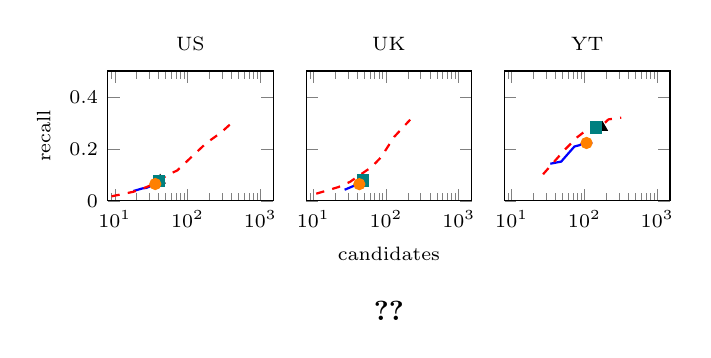
\begin{tikzpicture}
\begin{groupplot}[
  group style={group size=3 by 1, horizontal sep=0.42cm},
  scale only axis, width=2.10cm, height=1.65cm,
  xmode=log, log basis x=10,
  xlabel style={font=\scriptsize}, ylabel style={font=\scriptsize},
  tick label style={font=\scriptsize},
  title style={font=\scriptsize, yshift=-2pt},
  ymin=0, ymax=0.5, xmin=8, xmax=1500,
  legend style={font=\scriptsize, anchor=north, legend columns=3, /tikz/column sep=3pt},
]
\nextgroupplot[title={US}, ylabel={recall},
  legend to name=paretolegend]
\addplot[thick, blue] coordinates {(38,0.0678) (36,0.0650) (35,0.0636) (34,0.0618) (28,0.0514) (27,0.0500) (24,0.0481) (18,0.0379)};
\addlegendentry{$\theta$ sweep}
\addplot[thick, red, dashed] coordinates {(9,0.0175)(18,0.0351)(27,0.0526)(36,0.0682)(54,0.1013)(72,0.1169)(108,0.1636)(180,0.2220)(288,0.2629)(432,0.3072)};
\addlegendentry{ranked union}
\addplot[only marks, mark=triangle*, black] coordinates {(42,0.0793)};
\addlegendentry{Q}
\addplot[only marks, mark=square*, teal] coordinates {(40,0.0765)};
\addlegendentry{QS}
\addplot[only marks, mark=*, orange] coordinates {(36,0.0650)};
\addlegendentry{DIB}
\nextgroupplot[title={UK}, yticklabels=\empty, xlabel={candidates}]
\addplot[thick, blue] coordinates {(43,0.0644) (41,0.0631) (40,0.0631) (39,0.0618) (38,0.0605) (27,0.0428)};
\addplot[thick, red, dashed] coordinates {(11,0.0277)(22,0.0529)(32,0.0731)(43,0.0983)(64,0.1311)(86,0.1689)(129,0.2458)(215,0.3126)};
\addplot[only marks, mark=triangle*, black] coordinates {(48,0.0784)};
\addplot[only marks, mark=square*, teal] coordinates {(48,0.0784)};
\addplot[only marks, mark=*, orange] coordinates {(43,0.0644)};
\nextgroupplot[title={YT}, yticklabels=\empty]
\addplot[thick, blue] coordinates {(129,0.2229)(122,0.2229)(107,0.2229)(97,0.2229)(86,0.2146)(73,0.2094)(58,0.1778)(48,0.1513)(34,0.1430)};
\addplot[thick, red, dashed] coordinates {(27,0.1023)(54,0.1978)(80,0.2455)(107,0.2728)(160,0.2796)(214,0.3137)(321,0.3205)};
\addplot[only marks, mark=triangle*, black] coordinates {(177,0.2823)};
\addplot[only marks, mark=square*, teal] coordinates {(146,0.2823)};
\addplot[only marks, mark=*, orange] coordinates {(107,0.2229)};
\end{groupplot}
\node at ($(group c2r1.south)+(0,-1.4cm)$) {\ref{paretolegend}};
\end{tikzpicture}
\caption{Candidate count and macro recall for cold-start receivers. Solid curves vary $\theta\in[0.50,0.80]$ at $m=2$; dashed curves rank the pooled union by score at increasing budgets. Scores use raw breadth.}
\label{fig:pareto}
\end{figure}

DIB reduces candidate counts by 96.4\% at US, 94.4\% at UK, and 92.3\% at YT, but this reduction sacrifices coverage. The full union contains more receiver-observed endpoints---184/178/49 among 1005/767/1387 candidates---and achieves higher macro F1 at US/UK. It also requires 5.46/4.31/28.31 inspected entries per receiver-observed endpoint, compared with DIB's 1.03/1.16/2.89. At the smaller DIB budgets, unranked union yields only an expected 6.6/10.0/3.8 matching endpoints.

Ordering alone nevertheless recovers much of the review yield. At DIB's budgets of 36/43/107 candidates, ranking the full union yields 35/39/40 receiver-observed endpoints, compared with DIB's 35/37/37. The ranked prefixes overlap DIB's queues by 86.9--90.7\%; the additional matching endpoints at UK and YT pass quorum and score but fail endpoint eligibility. Quorum supplies most of the reduction at US/UK, yielding 35.1/36.7 matching endpoints at the DIB budgets. At YT, yield rises from 24.8 with quorum to 30.0 with quorum and score and 37.0 with the full rule.

Admission and ordering thus serve different purposes: ranking limits review to a budget, whereas admission excludes adversary-only evidence under the raw-breadth Criterion~\ref{crit:poison-bound}. We recommend \emph{threshold-then-rank} when that condition holds, reviewing a score-ordered prefix of the admitted queue when the budget is smaller than the queue. Figure~\ref{fig:pareto} distinguishes these choices: solid curves vary the admission threshold and show its effect on queue size and recall; dashed curves rank the full union at increasing budgets. The solid curves do not evaluate prefixes of a fixed admitted queue.


These comparisons describe filter behavior on the selected captures, not a ranking of receiving environments. Observation windows and endpoint-set sizes differ, and only six device types are common to all three deployments. Their 95\% F1 intervals (Table~\ref{tab:threelab}), computed by percentile bootstrap over those six types (1,000 resamples, seed 42), overlap across receivers. Restricting US and UK to their busiest days gives macro F1 0.241/0.213/0.258, further illustrating sensitivity to the observation window.


\subsection{Adversarial Observations and Fabricated Evidence}
\label{sec:security-results}
Captured malicious traffic and fabricated reports challenge admission in different ways. We inject both into the ten UNSW pseudo-sites, whose partition fixes the reporting population and lets us control the raw malicious breadth share $f_s$ of Criterion~\ref{crit:poison-bound}. This setup does not establish reporter independence in a real consortium; that remains a governance assumption (Sec.~\ref{subsec:trust}). The tests include 59 captured A1 facts at $k=1,\ldots,10$ pseudo-sites, resolved-name and port-masquerading fabrications, and A2 across 20 seeds and malicious-site fractions $\{.05,.1,.2,.3,.4,.5\}$, realized by uniformly sampling the rounded pseudo-site count.

DIB stages none of the 59 captured A1 facts; pooled union and frequency filtering stage all of them. Five annotation logs contain 354 packets with IP-literal destinations. Retaining device-originated packets with recognized transport protocols yields 165 observations and 59 endpoint facts. Replacing IPs with resolvable names, with devices, sites, and timing unchanged, raises admission from 0/150 to 21/150 configurations: five device types, $k=1,\ldots,10$ reporting sites, and spread windows of 1, 30, or 120 days. Admission first occurs at $k=7$ over 120 days (score 0.679). The filter rejects unresolved infrastructure, not malicious behavior in general: resolved attacker domains can enter review.

Port masquerading exposes the same distinction. With other inputs fixed, ports 53/123 pass endpoint eligibility while the port-443 control fails. At a one-day horizon, this counterfactual and the bounded-A2 tests share a maximum score of 0.354; extending fabrication to 120 days exceeds that value. These masquerading runs use the selected trust-weighted configuration (seed 42, ten pseudo-sites). At $f_s=0.30$, the largest score passing quorum is 0.562 over 120 days, below $\theta$. This is the maximum of the tested strategy, not of the threat model: the bound of Criterion~\ref{crit:poison-bound} is 0.58 under raw breadth, and an exhaustive worst case with raw breadth, three adversarial sites out of ten reporting on every active day of each UNSW device type, reaches 0.579. At $f_s=0.50$, outside the assumed bound, a 30-day fabrication reaches 0.663 under trust weighting and enters MonitorOnly. Thus, failure of admission filtering creates a false proposal, not permission to communicate.

\subsubsection{Parameter Sensitivity, Identity Inflation, and Drift}
\label{sec:sensitivity-results}
The operating point chosen from the adversarial bound is not the one that maximizes traffic agreement. Sweeping $\theta\in[0.50,0.80]$ and $\alpha\in[0.4,0.9]$ on Mon(IoT)r yields a best macro F1 of 0.071, compared with 0.054 at the chosen setting. Figure~\ref{fig:pareto} reports the separate cold-start threshold sweep at fixed $m=2$.

Identity inflation deliberately violates the malicious-share assumption. The test grid uses 200--3,200 fabricated identities over 20--400 days, diversifying endpoint sets by 0--50\% of a baseline pool. Raw counting admits the fabrication in 45 of 48 representative configurations. Trust weighting and clustering reject those configurations, while RWV admits all 48 at its fixed operating point. That protection is not universal: padding fabricated identities with real endpoints defeats clustering in the extreme configuration (score 0.905), and no tested Jaccard threshold in $[0.6,0.95]$ withstands every padding level.

Even without identity inflation, identical observations cannot reveal different intentions. A synthetic rollout tests all $27\times6=162$ device-type/adoption pairs, with $p\in\{.2,.4,.5,.6,.8,1\}$, at each duration $D\in\{1,7,30,120\}$ days; 69 pairs enter review at $D=120$. A separate time-to-admission sweep samples the same rollout at days 1, 3, 7, 14, 30, 60, 90, and 120. Among the 69 pairs admitted by day 120, the median first-admission checkpoint is seven days. Labeling an injected endpoint as legitimate change or compromise produces identical scores. Existing Active facts remain authorized with only a review flag. Distinguishing a rollout from a slow compromise with identical endpoints and cadence therefore requires operator review or out-of-band investigation.



\section{Discussion}
\label{sec:discussion}

Recovery requires approval validity and revocation origin, whether represented through states or history. The mutations (Table~\ref{tab:tla}) and restoration-policy ablation (Table~\ref{tab:comparison}) expose failures when this information or its checks are omitted. The review process still requires evaluation with operators.

Candidate selection can adapt without changing local authorization or recovery. Quorum accounts for most queue reduction at US/UK; ordering explains the advantage over unranked pooling. Threshold-then-rank suits deployments that maintain the bounded raw-breadth share assumption of Criterion~\ref{crit:poison-bound}. Trust weighting and clustering mitigate tested identity inflation but fail under padding. Ranked union yields slightly more receiver-observed endpoints at matched budgets, but no tested policy establishes benignity or necessity. Review capacity should inform the retention window $W$, whose practical value remains open.

Local control does not eliminate withdrawal's availability costs. One reporter can interrupt service under immediate suspension; requiring two preserves permissions until corroboration but delays withdrawal if no second report arrives. Both policies remain vulnerable to collusion, and the prototype lacks dispute rate limits and reputation penalties. Unreachable gateways can retain stale rules until reconnection, with no established withdrawal deadline. Operators need visibility into pending updates and installed policies; rule leases could bound stale permissions at an additional availability cost.

The shared evidence service is a throughput bottleneck and single point of failure for candidate flow and withdrawal propagation. It holds no local authorization state: failure can delay withdrawal but cannot itself grant or revoke local permissions. Replication and recovery remain deployment concerns. Co-located experiments emulate delay and loss on one host pair rather than measure a real wide-area network, and do not evaluate production workloads; finite models assume authenticated callers, and gateway tests disable signature validation. Deployment requires the authentication, roles, and signing integration in Sec.~\ref{subsec:trust}.

The pseudo-site partition and six-type alignment restrict generalization. Historical captures expose names through DNS or HTTP/TLS metadata. Encrypted Client Hello protects the inner server name, and encrypted DNS removes another source of name-to-address associations~\cite{rfc9849}; QUIC carries the TLS handshake in QUIC frames~\cite{rfc9001}. Coverage of fleets using these mechanisms remains unverified. Resolver-side telemetry or endpoint instrumentation could supply missing names without changing approval and recovery rules.

Policy output is similarly scoped: the exporter emits resolved-name TCP/UDP ACEs, not the TLS/DTLS profile parameters added by RFC~9761~\cite{rfc9761}. If a manufacturer profile later becomes available, it remains separate from locally approved facts, with the MUD manager combining the sources under deny-overrides. Reconciling them with authorized MUD-URL updates~\cite{mudacceptableurls} remains future work.



\section{Conclusion}
\label{sec:conclusion}
This paper presented DIB for managing locally authorized MUD policies from shared IoT observations. Finite-model checks and guard-removal mutations assess its authorization lifecycle; OpenWrt/osMUD tests demonstrate enforcement. Outage experiments show that one collapsed update preserves local vetoes and invalidates stale approvals after a missed withdrawal and restoration episode. Candidate-selection and suspension experiments quantify review volume and availability costs. Future work will evaluate operator review, mechanisms to bound gateway withdrawal time, and recovery of the shared evidence service.



\begin{thebibliography}{00}

\bibitem{mirai} M. Antonakakis \emph{et al.}, ``Understanding the Mirai Botnet,'' in
\emph{Proc. 26th USENIX Security Symp.}, 2017, pp. 1093--1110.

\bibitem{lamport1982byzantine} L. Lamport, R. Shostak, and M. Pease, ``The Byzantine Generals Problem,'' \emph{ACM Trans. Program. Lang. Syst.}, vol. 4, no. 3, pp. 382--401, 1982.

\bibitem{castro1999pbft} M. Castro and B. Liskov, ``Practical Byzantine Fault Tolerance,'' in \emph{Proc. 3rd USENIX Symp. Operating Systems Design and Implementation (OSDI)}, New Orleans, LA, USA, Feb. 1999, pp. 173--186.

\bibitem{kumar2019allthings} D. Kumar, K. Shen, B. Case, D. Garg, G. Alperovich, D. Kuznetsov, R. Gupta, and Z. Durumeric, ``All Things Considered: An Analysis of IoT Devices on Home Networks,'' in \emph{Proc. 28th USENIX Security Symp.}, 2019, pp. 1169--1185.

\bibitem{zhao2022largescale} B. Zhao, S. Ji, W.-H. Lee, C. Lin, H. Weng, J. Wu, P. Zhou, L. Fang, and R. Beyah, ``A Large-Scale Empirical Study on the Vulnerability of Deployed IoT Devices,'' \emph{IEEE Trans. Dependable Secure Comput.}, vol. 19, no. 3, pp. 1826--1840, May/Jun. 2022.

\bibitem{rfc8520} E. Lear, R. Droms, and D. Romascanu, ``Manufacturer Usage Description
Specification,'' RFC 8520, IETF, Mar. 2019.

\bibitem{clearasmud} A. Hamza, D. Ranathunga, H. Habibi Gharakheili, M. Roughan, and
V. Sivaraman, ``Clear as MUD: Generating, Validating and Applying IoT Behavioral
Profiles,'' in \emph{Proc. ACM SIGCOMM Workshop IoT S\&P}, 2018.

\bibitem{sivanathan2019classifying} A. Sivanathan \emph{et al.}, ``Classifying IoT Devices
in Smart Environments Using Network Traffic Characteristics,'' \emph{IEEE Trans. Mobile
Comput.}, vol. 18, no. 8, pp. 1745--1759, 2019.

\bibitem{hamzatdsc} A. Hamza \emph{et al.}, ``Verifying and Monitoring IoTs Network
Behavior Using MUD Profiles,'' \emph{IEEE Trans. Dependable Secure Comput.}, vol. 19, no.
1, pp. 1--18, 2022.

\bibitem{mudflow} A. Hamza, H. Habibi Gharakheili, T. A. Benson, and V. Sivaraman,
``Detecting Volumetric Attacks on IoT Devices via SDN-Based Monitoring of MUD Activity,''
in \emph{Proc. ACM SOSR}, 2019.

\bibitem{CornoMannella2023GatewayMUD} F. Corno and L. Mannella, ``A Gateway-based MUD
Architecture to Enhance Smart Home Security,'' in \emph{Proc. SpliTech}, 2023, pp. 1--6.

\bibitem{osmud} osMUD Project, ``osMUD: Open Source MUD Manager,''
\url{https://osmud.org}. (Accessed Jul. 24, 2026.)

\bibitem{hernandezramos2021mudreview} J. L. Hern\'andez-Ramos, S. N. Matheu,
A. Feraudo, G. Baldini, J. Bernal Bernabe, P. Yadav, A. Skarmeta, and
P. Bellavista, ``Defining the Behavior of IoT Devices Through the MUD Standard:
Review, Challenges, and Research Directions,'' \emph{IEEE Access}, vol. 9,
pp. 126265--126285, 2021.

\bibitem{matheu2019mudtesting} S. N. Matheu, J. L. Hern\'andez-Ramos, S. P\'erez,
and A. F. Skarmeta, ``Extending MUD Profiles Through an Automated IoT Security
Testing Methodology,'' \emph{IEEE Access}, vol. 7, pp. 149444--149463, 2019.

\bibitem{ndiot2019} T. D. Nguyen \emph{et al.}, ``D\"IoT: A Federated Self-learning Anomaly
Detection System for IoT,'' in \emph{Proc. IEEE ICDCS}, 2019, pp. 756--767.

\bibitem{vasilomanolakis2015collaborative} E. Vasilomanolakis, S. Karuppayah,
M. M\"uhlh\"auser, and M. Fischer, ``Taxonomy and Survey of Collaborative Intrusion
Detection,'' \emph{ACM Comput. Surv.}, vol. 47, no. 4, Art. 55, 2015.

\bibitem{colearn} A. Feraudo, P. Yadav, V. Safronov, D. A. Popescu, R. Mortier,
S. Wang, P. Bellavista, and J. Crowcroft, ``CoLearn: Enabling Federated Learning
in MUD-Compliant IoT Edge Networks,'' in \emph{Proc. ACM EdgeSys}, 2020,
pp. 25--30.

\bibitem{mudscope} L. Morgese Zangrandi, T. van Ede, T. Booij,
S. Sciancalepore, L. Allodi, and A. Continella, ``Stepping out of the MUD:
Contextual Threat Information for IoT Devices with Manufacturer-Provided
Behavior Profiles,'' in \emph{Proc. ACSAC}, 2022, pp. 467--480.

\bibitem{wagner2016misp} C. Wagner, A. Dulaunoy, G. Wagener, and A. Iklody, ``MISP: The
Design and Implementation of a Collaborative Threat Intelligence Sharing Platform,'' in
\emph{Proc. ACM WISCS}, 2016, pp. 49--56.

\bibitem{stix21} OASIS CTI TC, ``STIX Version 2.1,'' OASIS Standard, Jun. 2021.

\bibitem{eigentrust} S. D. Kamvar, M. T. Schlosser, and H. Garcia-Molina, ``The EigenTrust
Algorithm for Reputation Management in P2P Networks,'' in \emph{Proc. WWW}, 2003.

\bibitem{trustsurvey} A. J\o{}sang, R. Ismail, and C. Boyd, ``A Survey of Trust and
Reputation Systems for Online Service Provision,'' \emph{Decision Support Systems}, vol.
43, no. 2, pp. 618--644, 2007.

\bibitem{pbnm} M. Sloman, ``Policy Driven Management for Distributed Systems,'' \emph{J.
Netw. Syst. Manage.}, vol. 2, no. 4, pp. 333--360, 1994.

\bibitem{rfc9315} A. Clemm, L. Ciavaglia, L. Z. Granville, and J. Tantsura,
``Intent-Based Networking: Concepts and Definitions,'' RFC 9315, IETF, Oct. 2022.

\bibitem{alshaer2004firewall} E. Al-Shaer and H. Hamed, ``Modeling and Management of
Firewall Policies,'' \emph{IEEE Trans. Netw. Serv. Manage.}, vol. 1, no. 1, pp. 2--10,
Apr. 2004, doi: 10.1109/TNSM.2004.4623689.

\bibitem{chowdhary2022intent} A. Chowdhary, A. Sabur, N. Vadnere, and D. Huang,
``Intent-Driven Security Policy Management for Software-Defined Systems,''
\emph{IEEE Trans. Netw. Serv. Manage.}, vol. 19, no. 4, pp. 5208--5223, 2022,
doi: 10.1109/TNSM.2022.3183591.

\bibitem{pipeconf2022} A. dos Santos Pires, F. M. Matos, A. Santos, D. Pessoa,
\emph{et al.}, ``PipeConf: An Integrated Architecture for the Automated
Configuration of Network Assets,'' \emph{IEEE Trans. Netw. Serv. Manage.},
vol. 19, no. 3, Sep. 2022, doi: 10.1109/TNSM.2022.3195382.

\bibitem{vergutz2023data} A. Verg\"utz, B. V. dos Santos, B. Kantarci, and
M. Nogueira, ``Data Instrumentation From IoT Network Traffic as Support for
Security Management,'' \emph{IEEE Trans. Netw. Serv. Manage.}, vol. 20, no. 2,
pp. 1392--1404, Jun. 2023, doi: 10.1109/TNSM.2022.3233673.

\bibitem{blockchainmud} C. K. Rath, A. K. Mandal, and A. Sarkar, ``Blockchain-based
Dynamic MUD Profiles for Tamper-proof IoT Access Control,'' \emph{J. Inf. Secur. Appl.},
vol. 95, Art. 104273, 2025, doi: 10.1016/j.jisa.2025.104273.

\bibitem{moniotr} J. Ren, D. J. Dubois, D. Choffnes, A. M. Mandalari, R. Kolcun, and
H. Haddadi, ``Information Exposure From Consumer IoT Devices: A Multidimensional,
Network-Informed Measurement Approach,'' in \emph{Proc. ACM IMC}, 2019,
pp. 267--279, doi: 10.1145/3355369.3355577.

\bibitem{alrawi2019yourthings} O. Alrawi, C. Lever, M. Antonakakis, and F. Monrose,
``SoK: Security Evaluation of Home-Based IoT Deployments,'' in \emph{Proc. IEEE
Symp. Security and Privacy}, 2019.

\bibitem{iotinspector} D. Y. Huang, N. Apthorpe, F. Li, G. Acar, and N. Feamster,
``IoT Inspector: Crowdsourcing Labeled Network Traffic from Smart Home Devices at
Scale,'' \emph{Proc. ACM Interact. Mob. Wearable Ubiquitous Technol.}, vol. 4,
no. 2, Art. 46, 2020.

\bibitem{allowlistvariability} W. He, K. Bryson, R. Calderon, V. Prakash,
N. Feamster, D. Y. Huang, and B. Ur, ``Can Allowlists Capture the Variability
of Home IoT Device Network Behavior?'' in \emph{Proc. IEEE EuroS\&P}, 2024,
pp. 114--138, doi: 10.1109/EuroSP60621.2024.00015.

\bibitem{rfc9761} T. Reddy.K, D. Wing, and B. Anderson, ``Manufacturer Usage Description
(MUD) for TLS and DTLS Profiles for IoT Devices,'' RFC 9761, IETF, Apr. 2025.

\bibitem{fidem} A. Lotto, S. Sciancalepore, A. Brighente, and M. Conti, ``FIDEM: A
Standard-Compliant Framework for Secure Binding of MUD Profiles to IoT Devices,''
\emph{arXiv preprint arXiv:2605.29654}, May 2026.

\bibitem{polaris} A. Zhang, X. Lee, Z. Zhuang, J. Wei, Y. Fu, and B. Peng, ``POLARIS:
Cross-Domain Access Control via Verifiable Identity and Policy-Based Authorization,''
in \emph{Proc. IEEE 24th Int. Conf. Trust, Security and Privacy in Computing and
Communications (TrustCom)}, 2025, pp. 1489--1498.

\bibitem{zanzibar} R. Pang \emph{et al.}, ``Zanzibar: Google's Consistent, Global
Authorization System,'' in \emph{Proc. USENIX Annu. Tech. Conf. (ATC)}, 2019,
pp. 33--46.

\bibitem{mudacceptableurls} M. Richardson, W. Pan, and E. Lear, ``Authorized
Update to MUD URLs,'' IETF Internet-Draft
\texttt{draft-ietf-iotops-mud-acceptable-urls}, work in progress, 2025.

\bibitem{xacml3} OASIS, ``eXtensible Access Control Markup Language (XACML)
Version 3.0,'' OASIS Standard, Jan. 2013.

\bibitem{ponder} N. Damianou, N. Dulay, E. Lupu, and M. Sloman, ``The Ponder
Policy Specification Language,'' in \emph{Proc. IEEE Int. Workshop on Policies
for Distributed Systems and Networks (POLICY)}, 2001, pp. 18--38.

\bibitem{crdt} M. Shapiro, N. Preguica, C. Baquero, and M. Zawirski,
``Conflict-Free Replicated Data Types,'' in \emph{Proc. Int. Symp. Stabilization,
Safety, and Security of Distributed Systems (SSS)}, 2011, pp. 386--400.

\bibitem{rfc9849} E. Rescorla, K. Oku, N. Sullivan, and C. A. Wood,
``TLS Encrypted Client Hello,'' RFC 9849, IETF, Mar. 2026.

\bibitem{rfc9001} M. Thomson and S. Turner, ``Using TLS to Secure QUIC,''
RFC 9001, IETF, May 2021.

\end{thebibliography}


% \makeatletter
% \def\@IEEEBIOphotowidth{0.74in}
% \def\@IEEEBIOphotodepth{0.58in}
% \def\@IEEEBIOhangwidth{0.84in}
% \def\@IEEEBIOhangdepth{0.58in}
% \def\@IEEEBIOskipN{0.05\baselineskip}
% \makeatother
% \begin{IEEEbiography}[{{\fbox{\rule{0pt}{0.52in}\rule{0.62in}{0pt}}}}]{Author One}
% received the Ph.D. degree in [field] from [university] in [year]. [He/She/They] is currently [position] at [institution]. Research interests include [topic one], [topic two], and [topic three].
% \end{IEEEbiography}
% \begin{IEEEbiography}[{{\fbox{\rule{0pt}{0.52in}\rule{0.62in}{0pt}}}}]{Author Two}
% received the Ph.D. degree in [field] from [university] in [year]. [He/She/They] is currently [position] at [institution]. Research interests include [topic one], [topic two], and [topic three].
% \end{IEEEbiography}
% \begin{IEEEbiography}[{{\fbox{\rule{0pt}{0.52in}\rule{0.62in}{0pt}}}}]{Author Three}
% received the Ph.D. degree in [field] from [university] in [year]. [He/She/They] is currently [position] at [institution]. Research interests include [topic one], [topic two], and [topic three].
% \end{IEEEbiography}
% \begin{IEEEbiography}[{{\fbox{\rule{0pt}{0.52in}\rule{0.62in}{0pt}}}}]{Author Four}
% received the Ph.D. degree in [field] from [university] in [year]. [He/She/They] is currently [position] at [institution]. Research interests include [topic one], [topic two], and [topic three].
% \end{IEEEbiography}
% \begin{IEEEbiography}[{{\fbox{\rule{0pt}{0.52in}\rule{0.62in}{0pt}}}}]{Author Five}
% received the Ph.D. degree in [field] from [university] in [year]. [He/She/They] is currently [position] at [institution]. Research interests include [topic one], [topic two], and [topic three].
% \end{IEEEbiography}
% \begin{IEEEbiography}[{{\fbox{\rule{0pt}{0.52in}\rule{0.62in}{0pt}}}}]{Author Six}
% received the Ph.D. degree in [field] from [university] in [year]. [He/She/They] is currently [position] at [institution]. Research interests include [topic one], [topic two], and [topic three].
% \end{IEEEbiography}
% \begin{IEEEbiography}[{{\fbox{\rule{0pt}{0.52in}\rule{0.62in}{0pt}}}}]{Author Seven}
% received the Ph.D. degree in [field] from [university] in [year]. [He/She/They] is currently [position] at [institution]. Research interests include [topic one], [topic two], and [topic three].
% \end{IEEEbiography}

\end{document}